\documentclass[11pt]{article}
\usepackage[margin=1in]{geometry}
\usepackage[T1]{fontenc}
\usepackage{amsmath,amssymb}
\usepackage{graphicx}
\usepackage{booktabs,tabularx,longtable,array,multirow}
\usepackage{xcolor}
\usepackage{tikz}
\usetikzlibrary{arrows.meta,positioning,calc,fit,backgrounds}
\usepackage[numbers,sort&compress]{natbib}
\usepackage[hidelinks]{hyperref}
\usepackage{xurl}
\usepackage{enumitem}
\usepackage{caption}
\usepackage[most]{tcolorbox}
\newtcolorbox{keybox}[1]{colback=acc!5,colframe=acc!60,fonttitle=\bfseries,title=#1,boxrule=0.6pt,arc=2pt}
\setlist{itemsep=2pt,topsep=4pt}
\captionsetup{font=small,labelfont=bf}
\definecolor{nb}{HTML}{2A78D6}\definecolor{sb}{HTML}{EB6834}\definecolor{single}{HTML}{D6962C}
\definecolor{ink}{HTML}{1D2622}\definecolor{muted}{HTML}{6B736E}\definecolor{acc}{HTML}{0F6E66}
\newcolumntype{L}{>{\raggedright\arraybackslash}X}
\graphicspath{{figures/}}

\title{Running the River LINE with the Cars You Have:\\
\large Data, Timetables, Models, and a Decision Dashboard for NJ TRANSIT's Camden--Trenton Light Rail}
\author{ISE Senior Design Team 22 \quad (faculty advisor: R.~Hildebrand)\\Grado Department of Industrial and Systems Engineering, Virginia Tech}
\date{Working report --- September 28, 2026 (revision 4: one headline measure, calibrated scenarios, validation)}

\begin{document}
\maketitle

\begin{abstract}
NJ TRANSIT's River LINE runs a weekday timetable that needs eight trains at the peaks, from an aging fleet that often cannot supply them. A breakdown also ties up a second car to rescue it. This report does five things:
\begin{enumerate}
\item assembles the public data on the line, including NJ TRANSIT's September 2026 timetable;
\item calibrates a single-track model against the places where that timetable schedules trains to pass;
\item analyzes the current timetable and builds proposed timetables, one for each number of available trains, with an optimizer that spaces trains as evenly as the single track allows;
\item simulates a year of operations under several ways of choosing the day's timetable from the 6\,am hold sheet;
\item proposes nine schedule changes and tests each with a delay-propagation simulation calibrated to NJ TRANSIT's reported on-time performance;
\item packages the results in an interactive dashboard with a playbook for dispatchers.
\end{enumerate}
The current timetable uses 8 trains in a 150-minute round trip and spaces them 15/15/30 minutes apart. A uniform 20-minute service would need 9 trains. An 8-train timetable with the same round trip can narrow the largest morning gap from 30 to 21 minutes, but the delay simulation shows that it packs the single-track meets and layovers so tightly that on-time performance falls from 84\% to 72\%: today's 30-minute gap works as recovery time. A robust 8-train timetable (B8: 160-minute cycle, at least 2.5 minutes of slack at every meet, 9-minute layovers) uses the same trains and train-hours and raises on-time performance to 87\% (79\% on a hot day, against 60\% today). A published summer timetable with 7 trains reaches 86\% on hot days.

Under placeholder failure parameters, running today's timetable with whatever cars are available cancels about 12\% of trips over a year and 21\% in summer. Publishing the proposed timetable that fits the morning car count, while holding one protect car, cancels about 2\%. The benefit comes from days with fewer than 9--10 cars and disappears if fleet reliability recovers.

\textbf{Revision 4} combines the fleet and delay simulations into one headline measure: on-time trip-miles delivered, as a share of today's timetable. It recalibrates the inputs to NJ TRANSIT and NTD data and tests the model against 2024--26 evidence (Section~\ref{sec:combined}). With the calibrated inputs, the fleet's reliability matters most: from the 2024--25 Alstom era to 2026 under NJ TRANSIT, the measure rises from 69\% to 84\%. Among schedule choices, the robust timetable B8 matters most, adding 3--4 points in every scenario at no extra cost. Choosing the day's timetable from the 6\,am car count adds about 1 point in the 2024--25 conditions and nothing at 2026 reliability. The earlier T8--T3 tiers score below today's timetable on this measure.
\end{abstract}

\tableofcontents
\newpage


%======================================================================
\section{Questions, measures, and results at a glance}\label{sec:glance}
\paragraph{The client's decision.} Given the cars available at 6\,am, what should the River LINE run today? And which timetables should NJ TRANSIT have ready?

\paragraph{Headline measure.} \emph{Reliable trip-miles delivered} (RTD): the trip-miles that actually run and arrive less than 6 minutes late, as a percentage of the trip-miles in NJ TRANSIT's normal published weekday timetable. A cancelled trip counts as not delivered, and a late trip as delivered late. A day that runs more trip-miles than today's timetable is capped at 100\%. RTD rewards running the promised service, and running it on time, in one number.

{\small
\begin{longtable}{@{}p{3.6cm}p{4.1cm}p{5.2cm}p{2.3cm}@{}}
\toprule
Question & Measures & Result (calibrated, revision 4) & Confidence \\ \midrule\endhead
Q1. Which timetables fit the single track for each number of trains? & Trains needed; single-track conflicts; longest and average gap; train-hours & Today's 15/15/30 pattern is why 8 trains suffice (even spacing needs 9). Conflict-free timetables exist for 3--8 trains, including the robust B8 and B7 (Sections~\ref{sec:tt}, \ref{sec:prop}). & Medium: siding positions are calibrated, not surveyed \\
Q2. How punctual is each timetable once delays spread? & Share of trips under 6 minutes late; average lateness; minutes held at single track & Today 83\% (2024--25 conditions) and 93\% (2026). B8: 88\% and 94\%. T8: 71\% and 87\% (Table~\ref{tab:rtd}). & Medium: fitted to averages; bad days overstated (Table~\ref{tab:valid}) \\
Q3. Publish one timetable, or choose from the 6\,am car count? & Share of trips cancelled; RTD; cost per day & At 2024--25 reliability, choosing robust tiers each morning cuts cancellations from 9.7\% to 2.4\% and raises RTD from 69\% to 74\%. B8 alone gives 73\%. At 2026 reliability, choosing adds nothing over B8 every day (both 87.5\%). & Low--medium: repair times inferred, cancellation records missing \\
Headline & RTD with range over 10 simulated years & B8 (or robust tiers) beats today in every scenario by 3--5 points at the same cost. Moving from 2024--25 to 2026 reliability is worth 13--18 points. & See Section~\ref{sec:combined} \\
\bottomrule
\end{longtable}}

\paragraph{Proposed targets} (to be agreed with NJ TRANSIT):
\begin{itemize}
\item RTD of at least 90\%;
\item on time at least 95\% (NJ TRANSIT's goal is 97\% \citep{news12_2025});
\item unplanned cancellations at most 1\%;
\item longest peak gap no worse than today (30 minutes);
\item no more train-hours than today (109 a weekday).
\end{itemize}
No option reaches the 90\% RTD target at today's fleet reliability. B8 on a renewed fleet comes closest (89.5\%), so reaching it needs both a better timetable and a more reliable fleet.

%======================================================================
\section{Summary for the client}
\begin{itemize}
\item \textbf{Today's schedule works because it is irregular.} The September 2026 timetable runs exactly 8 trains at the peaks and 6 midday. The 8 peak trains share a 150-minute round trip, with trains 15, 15 and 30 minutes apart. Even 20-minute spacing would need a 9th train, because the single-track meets would not fit (Sections~\ref{sec:today} and \ref{sec:ladder}).
\item \textbf{A more even 8-train timetable exists, but it runs late.} Our optimizer finds an 8-train pattern (T8) in the same 150-minute cycle with gaps of 17--21 minutes toward Trenton and the same train-hours. Every meet falls on double track (Section~\ref{sec:tt}). But T8 leaves little slack at meets and at the terminals, so one late train delays the next. In the delay simulation it is on time 72\% of trips against 84\% for today's timetable (Section~\ref{sec:prop}).
\item \textbf{Recommended weekday timetable: B8.} Same 8 trains and train-hours as today; a 160-minute cycle, at least 2.5 minutes of slack at every single-track meet and at least 9 minutes of layover. On time 87\% (79\% on a hot day, today 60\%), with wait plus lateness per rider unchanged. It gives up the even spacing: with 8 trains, even spacing and punctuality trade off, and B8 buys punctuality. B7 is its 7-train version.
\item \textbf{Publish a summer timetable.} W7 plans for heat speed restrictions (+6\% running time) with 7 trains: 86\% on time on hot days, and fewer cancellations in summer because an extra car is free.
\item \textbf{Moving running-time slack to the sidings did not help on its own.} Neither did longer layovers alone or meet buffers alone; both are needed (Figure~\ref{fig:propwhy}).
\item \textbf{Each car count gets its own conflict-free timetable.} T7 through T3 are timetables for 7 down to 3 trains, printed in the accompanying timetable book and shown on the dashboard.
\item \textbf{On short days, publish the timetable the cars can run.}
  \begin{itemize}
  \item With 5--6 cars, today's timetable run with whatever cars are available loses 25--40\% of trips in summer. The matching proposed timetable with a protect car loses 3--4\%.
  \item With 7--9 cars, the loss drops from 3.5--14\% to about 2.5\%.
  \item With 10 or more cars, keep today's timetable (Section~\ref{sec:playbook}).
  \end{itemize}
\item \textbf{The benefit depends on how often cars are short.} If breakdowns fall back to one per 8{,}000 miles, or repairs take about 6 days, today's timetable already cancels under 2\% and tiering adds little. The hold sheets will settle this.
\item \textbf{Three questions for NJ TRANSIT.}
  \begin{enumerate}
  \item Where exactly are the passing sidings? Public sources disagree with NJ TRANSIT's own timetable; we calibrated to the timetable.
  \item Why does midday use 6 trains for 30-minute service when 5 fit in the round trip? Our simulation suggests it is recovery time; proposal E5 shows what running 5 would cost.
  \item Can a reduced timetable be published by 6\,am?
  \end{enumerate}
\end{itemize}

%======================================================================
\section{The problem}\label{sec:problem}
The River LINE is a 34-mile diesel light rail line with 21 stations between the Entertainment Center in Camden and the Trenton Transit Center. According to NJDOT, 12.7 miles are single track, with passing sidings at Pennsauken, South Burlington, Florence, and Roebling \citep{njdot2021riverline}. Passenger trains run 5:45\,am--10:00\,pm and Conrail freight uses the line overnight \citep{njdot2021riverline}.

The 20 Stadler GTW cars date from 2002--2003 \citep{wiki_riverline}. Reported miles between breakdowns fell from about 22{,}300 in 2022 to about 4{,}200 in 2024 \citep{roinj2025riverline}. Peak service was cut in the summers of 2023 and 2024, and in 2024 NJ TRANSIT added supplemental buses \citep{inquirer2023,news12_2024}. On-time performance was 80--84\% in 2023--2025 \citep{njtod2025}. NJ TRANSIT took over operations from its contractor in 2025--2026 \citep{njt2025alstom}.

\paragraph{The decision.} Each morning a hold sheet lists the serviceable cars. The client asked for a model that chooses the day's schedule from that count, balancing on-time performance, level of service, and customer impact. Two features set this apart from textbook timetabling:
\begin{enumerate}
\item the number of cars is random and seasonal;
\item a failed car must be rescued by another car.
\end{enumerate}

%======================================================================
\section{Data}\label{sec:data}
Table~\ref{tab:data} lists the data used. The companion \emph{Data Sources and Provenance} document gives links, processing steps and trust levels. The companion \emph{Data Request} lists what only NJ TRANSIT can provide.

\begin{table}[ht]\centering\small
\begin{tabularx}{\textwidth}{@{}p{3.4cm}Lp{3.1cm}@{}}
\toprule
Data & What it gives us & Source \\
\midrule
GTFS schedule, Sept.~2026 & 87 weekday trips; times at all 21 stations; 12 vehicle blocks & \citet{njt2026gtfs} \\
GTFS schedule, 2014 & Track shape (33.6\,mi); a running-time baseline & \citet{njt2014gtfs} \\
NJDOT fact sheet & Single and double track by milepost; sidings; car capacity & \citet{njdot2021riverline} \\
OpenStreetMap & Posted speeds; track shared by both directions & \citet{osm2026} \\
NOAA GHCN-Daily & Daily weather at Trenton, 2015--2026 & \citet{noaa_ghcnd} \\
National Transit Database & Monthly ridership; breakdowns; cost per revenue hour & \citet{ntd_monthly,ntd_breakdowns,ntd_metrics} \\
DVRPC onboard survey (2010) & Trip purpose; access and egress modes & \citet{dvrpc2013riverline} \\
Station boardings (2024) & $\approx$5{,}600 weekday boardings & \citet{wiki_riverline} \\
\bottomrule
\end{tabularx}
\caption{Public data used.}\label{tab:data}
\end{table}

\paragraph{Findings about the data.}
\begin{itemize}
\item \textbf{Running times have not changed since 2014.} Both the 2014 and 2026 timetables take 67 minutes end to end. At posted speeds with no stops, the trip would take 46 minutes (Figure~\ref{fig:osm}).
\item \textbf{The published track layout does not match the timetable.} Section~\ref{sec:calib} shows that NJ TRANSIT's own timetable schedules meets on track that NJDOT's mileposts, as we map them, mark as single. OpenStreetMap disagrees with both around the Roebling siding.
\item \textbf{The NTD reports the River LINE as Hybrid Rail (mode YR).} Its operating cost was \$36.4 million in FY2024, \$952 per vehicle revenue hour, and 1.86 million trips (see the companion background report). The light rail row we used earlier for failures (about 17{,}000 car-miles per major failure in 2023--2024 \citep{ntd_breakdowns}) is Hudson--Bergen, not the River LINE, whose reported figure is 4{,}200 \citep{roinj2025riverline}.
\item \textbf{No public data give ridership by hour.} The model uses an assumed hourly profile.
\end{itemize}

\begin{figure}[ht]\centering
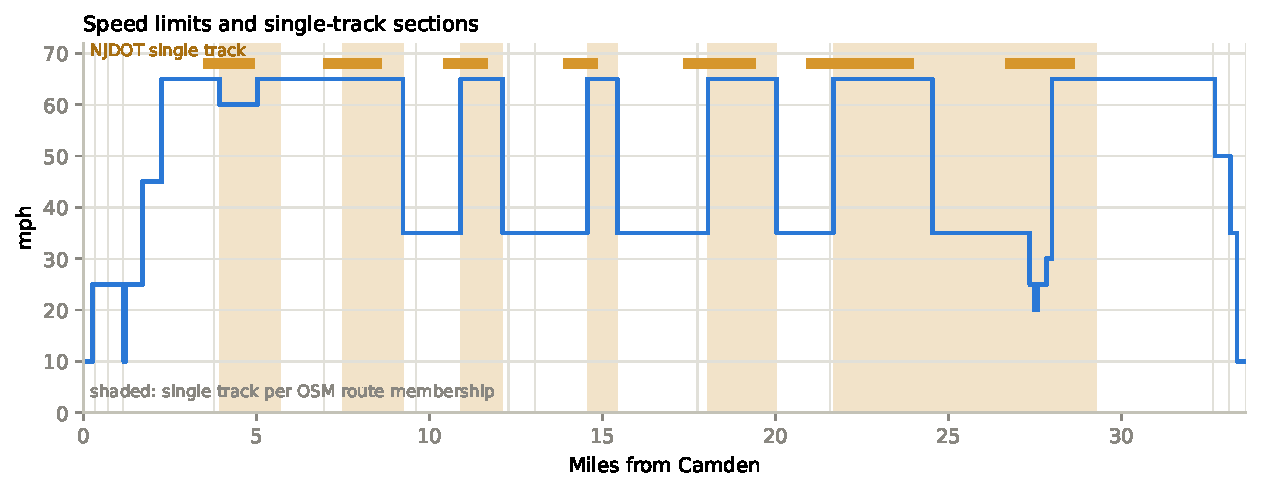
\includegraphics[width=\textwidth]{fig_osm_speed_track.pdf}
\caption{Posted speed toward Trenton (OpenStreetMap). Shaded: track shared by both directions in OpenStreetMap. Bars: single track per NJDOT, as mapped before calibration. Sources: \citet{osm2026,njdot2021riverline}.}\label{fig:osm}
\end{figure}

\subsection{Calibrating the track model to NJ TRANSIT's own meets}\label{sec:calib}
A timetable is only valid if opposing trains pass on double track. We therefore located every point where a northbound and a southbound trip cross in NJ TRANSIT's September 2026 weekday timetable, which gives 213 scheduled meets. They cluster at nine places: 0.4, 2.5, 6.6, 9.6, 13.3, 17.7, 21.6, 27.2 and 32.8 miles from Camden (Figure~\ref{fig:meets}).

The first five clusters fall on NJDOT double track. The meets at 17.7, 21.6 and 27.2 miles fall on sections that NJDOT's mileposts, rescaled to track distance, mark as single; 61 pairs of trips conflict. Shifting the mileposts north of MP~12 by 1.5 miles reduces this to one conflict, at the edge of the Pennsauken siding. The fit holds for any shift between 1.3 and 1.8 miles. Such an offset is plausible if the freight railroad's milepost zero is not the passenger terminal.

All models in this report use the calibrated layout. An official track chart should replace it.

\begin{figure}[ht]\centering
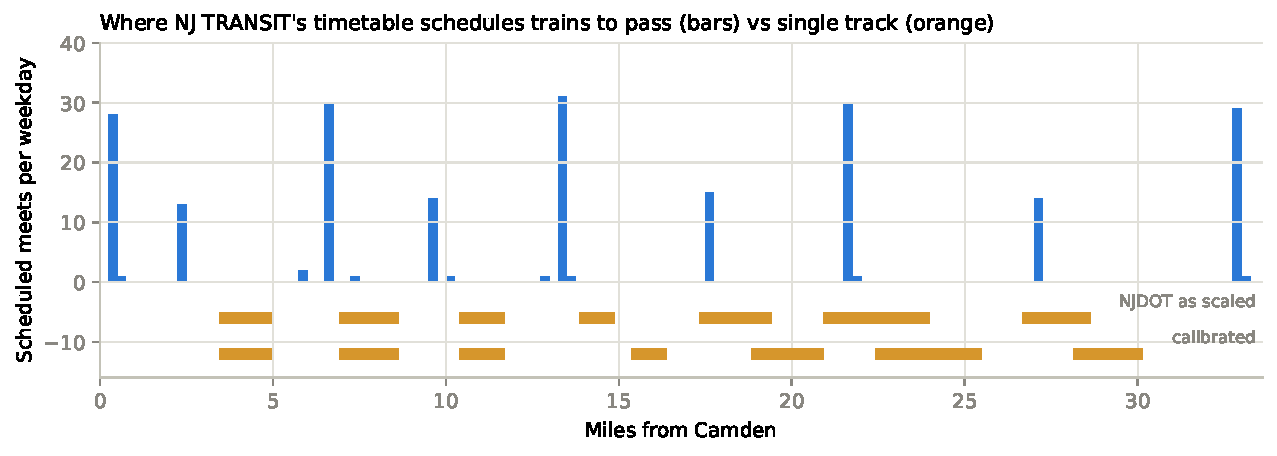
\includegraphics[width=\textwidth]{fig_meets_calibration.pdf}
\caption{Where the September 2026 timetable schedules trains to pass (bars), against single track before and after calibration (orange). Before calibration, three of the nine meet clusters sit on ``single'' track.}\label{fig:meets}
\end{figure}

%======================================================================
\section{What today's timetable does}\label{sec:today}
Figure~\ref{fig:gtfs} shows the September 2026 weekday timetable. The vehicle blocks show 8 trains at the peaks and 6 midday (Figure~\ref{fig:profile}).

\begin{figure}[ht]\centering
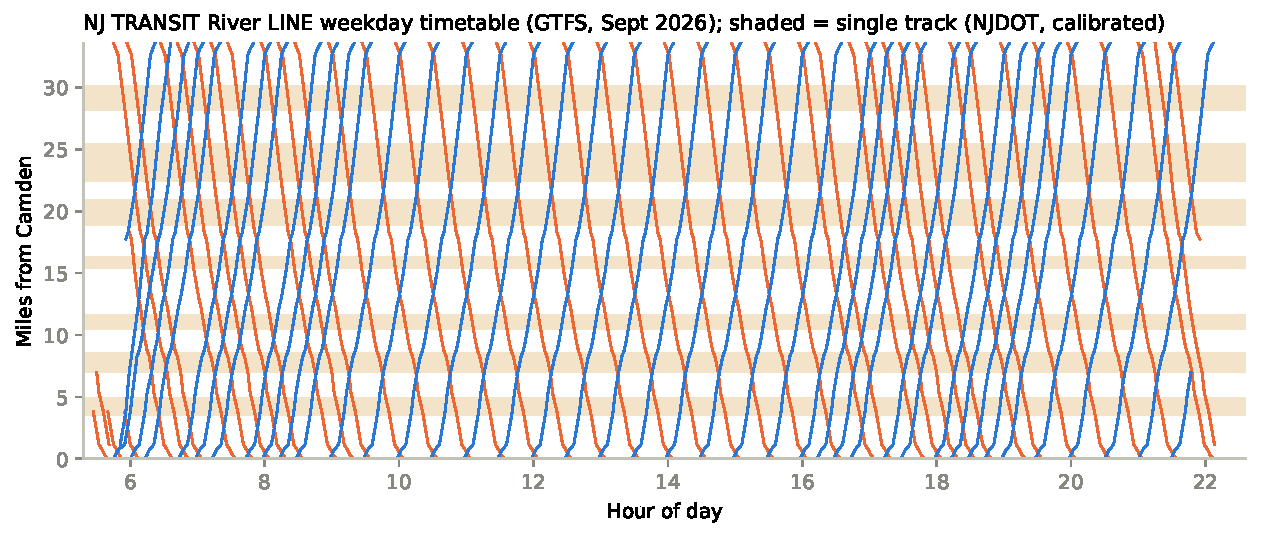
\includegraphics[width=\textwidth]{fig_gtfs_timespace.pdf}
\caption{NJ TRANSIT weekday timetable (GTFS, Sept.~15, 2026). Blue: toward Trenton; orange: toward Camden; shaded: single track (calibrated).}\label{fig:gtfs}
\end{figure}
\begin{figure}[ht]\centering
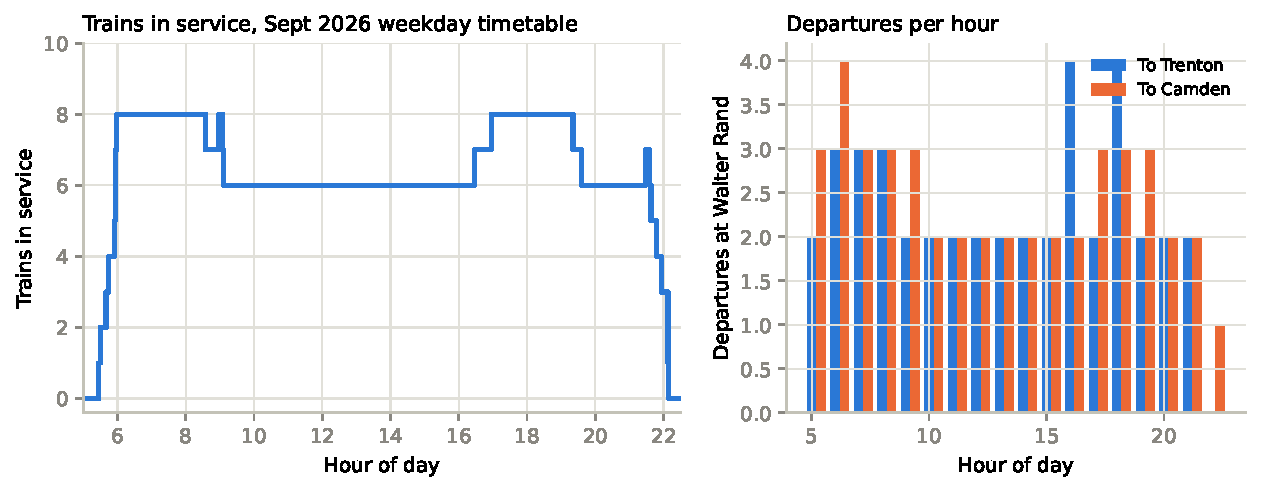
\includegraphics[width=\textwidth]{fig_gtfs_service_profile.pdf}
\caption{Trains in service (left) and departures per hour at Walter Rand (right).}\label{fig:profile}
\end{figure}

\paragraph{The 150-minute cycle.} Each peak train makes a round trip of 67 + 67 minutes of running plus about 16 minutes of turnback. Eight trains in 150 minutes allow an average of 18.75 minutes between trains. NJ TRANSIT spends that as 15, 15 and 30. With passengers arriving at random, the mean wait is
\begin{equation}\label{eq:wait}
\mathbb{E}[W]=\frac{\mathbb{E}[H]}{2}\bigl(1+\mathrm{CV}^2(H)\bigr)
\end{equation}
\citep{welding1957instability,osuna1972control}. At Walter Rand toward Trenton in the morning peak, this gives 9.6 minutes, against 8.75 minutes for the same trains evenly spaced.

\paragraph{Midday.} Six trains run every 30 minutes, which is a 180-minute cycle with long turnbacks. Five trains would fit a 150-minute cycle at 30 minutes. The sixth train may be deliberate recovery time, which is a question for the client.

%======================================================================
\section{Models}\label{sec:models}
\begin{figure}[ht]\centering
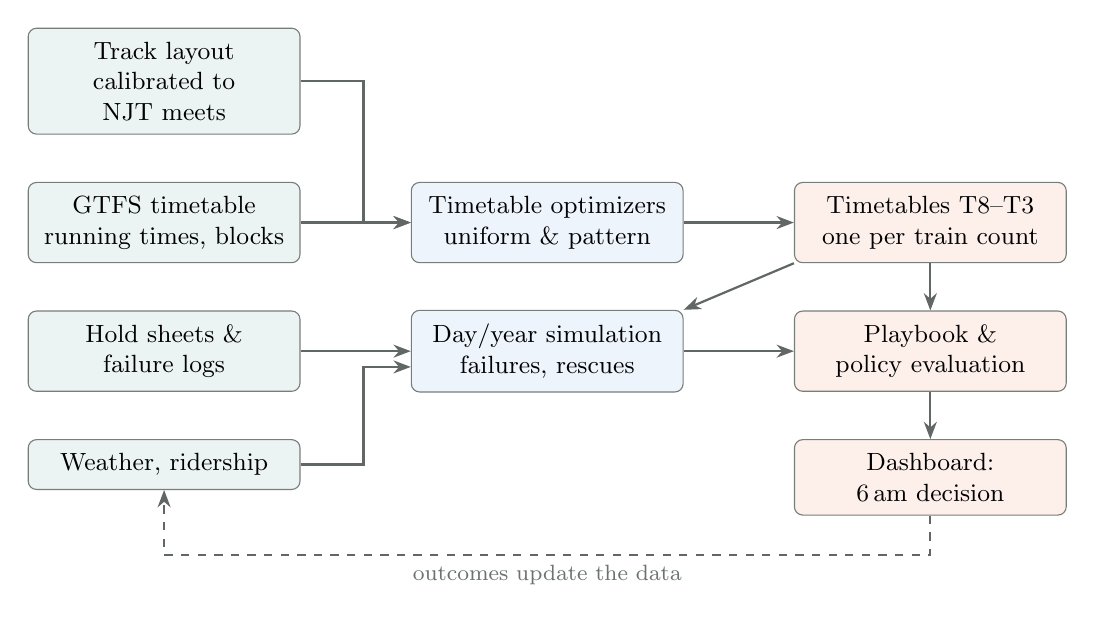
\begin{tikzpicture}[font=\small, node distance=6mm and 8mm,
  box/.style={draw=ink!60, rounded corners=3pt, align=center, inner sep=5pt, fill=white, text width=3.1cm},
  data/.style={box, fill=acc!8}, model/.style={box, fill=nb!8}, outb/.style={box, fill=sb!10},
  arr/.style={-{Stealth[length=2.2mm]}, thick, ink!70}]
\node[data] (track) {Track layout\\ calibrated to NJT meets};
\node[data, below=of track] (gtfs) {GTFS timetable\\ running times, blocks};
\node[data, below=of gtfs] (hold) {Hold sheets \&\\ failure logs};
\node[data, below=of hold] (wx) {Weather, ridership};
\node[model, right=14mm of gtfs] (mip) {Timetable optimizers\\ uniform \& pattern};
\node[model, right=14mm of hold] (sim) {Day/year simulation\\ failures, rescues};
\node[outb, right=14mm of mip] (tiers) {Timetables T8--T3\\ one per train count};
\node[outb, right=14mm of sim] (play) {Playbook \&\\ policy evaluation};
\node[outb, below=of play] (dash) {Dashboard: 6\,am decision};
\draw[arr] (track) -| ($(mip.west)+(-6mm,0)$) -- (mip.west);
\draw[arr] (gtfs) -- (mip);
\draw[arr] (hold) -- (sim);
\draw[arr] (wx.east) -| ($(sim.west)+(-6mm,-2mm)$) -- ($(sim.west)+(0,-2mm)$);
\draw[arr] (mip) -- (tiers); \draw[arr] (tiers) -- (play); \draw[arr] (sim) -- (play); \draw[arr] (tiers.south west) -- (sim.north east); \draw[arr] (play) -- (dash);
\draw[arr, dashed] (dash.south) -- ++(0,-5mm) -| node[pos=0.25, below, font=\footnotesize, text=muted]{outcomes update the data} (wx.south);
\end{tikzpicture}
\caption{How the pieces fit. Green: data; blue: models; orange: outputs.}\label{fig:pipeline}
\end{figure}

\subsection{Uniform-headway timetables}\label{sec:mip}
For a headway $T$, northbound trains leave Camden every $T$ minutes and southbound trains leave Trenton at offset $\phi$. Let $s$ be a single-track section, $o^N_s$ and $o^S_s$ the occupation times in each direction, $g=0.5$ minute a clearance buffer, and $p_s$, $q_s$ the entry times. The periodic event scheduling (PESP) form \citep{serafini1989mathematical} requires
\begin{equation}
0 \le q_s - p_s - o^N_s - g + T z_s \le T - o^N_s - o^S_s - 2g, \qquad z_s\in\mathbb{Z}.
\end{equation}
Trains may wait on double track, turnbacks need at least 5 minutes, and the round trip must equal $T m_C$. The integer $m_C$ is the number of trains, which the model minimizes. HiGHS solves each headway in under a second.

\subsection{Pattern timetables}\label{sec:pattern}
A uniform headway wastes trains whenever the round trip is not a multiple of $T$. The pattern model instead fixes the cycle $C$ (150 minutes, as today) and the number of trains $K$, and chooses each train's departure $a_k$ from Camden. Train $k$ leaves Trenton at
\[b_k=a_k+67+\textstyle\sum_d w^N_{kd}+\ell^T_k,\]
where $w^N_{kd}$ are its waits at double-track sections and $\ell^T_k \ge 5$ its Trenton turnback. It must be back in Camden by $a_k+C-5$.

Every pair of northbound train $i$ and southbound train $j$ on every single-track section $s$ gets the PESP constraint above with period $C$. The objective minimizes the sum of squared gaps in both directions, which by \eqref{eq:wait} is proportional to riders' average wait, plus a small penalty on siding waits. The square is linearized with tangent lines. For $K=8$ the model has 448 integer variables and solves within a minute.

To keep a day conflict-free, each proposed timetable runs one pattern all day. Off-peak, only the $k$ trains with the most even spacing keep running; the rest lay up after the morning peak and return for the evening peak. Any subset of a conflict-free pattern is itself conflict-free.

\subsection{Simulation}
The simulation is the same engine that runs in the dashboard. A day is a set of vehicle duties (blocks) taken from a timetable. Each duty is assigned a car at its start if one is free.
\begin{enumerate}
\item In-service failures occur at one per 4{,}192 car-miles \citep{roinj2025riverline}, scaled by season.
\item A failed car goes to the shop for a random repair time.
\item The rescue uses a protect car from where it waits, or failing that the nearest train in service, whose trips are cancelled while it helps.
\item A failure on single track blocks both directions.
\item Fleet availability carries over from day to day.
\end{enumerate}
The outputs are cancellations, on-time performance (within 6 minutes \citep{njt2019otp}), and waiting from \eqref{eq:wait} applied to the departures that actually run.

\begin{figure}[ht]\centering
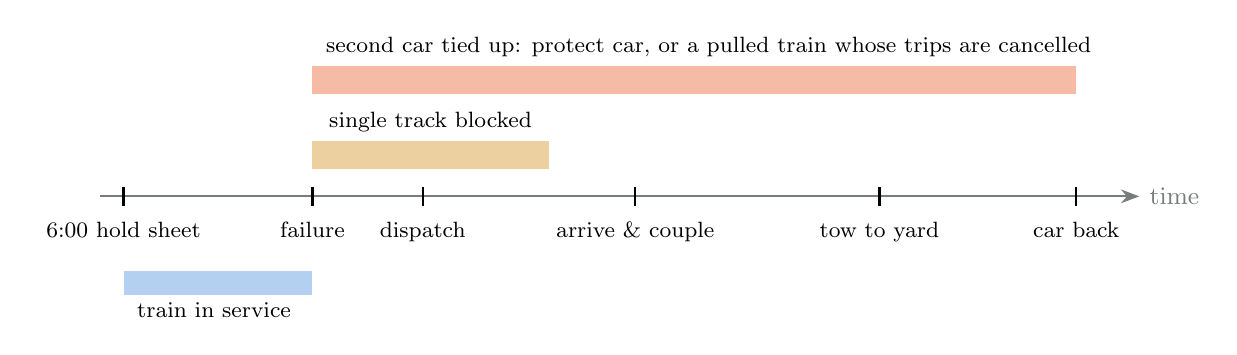
\begin{tikzpicture}[font=\small, >=Stealth]
\draw[->, thick, ink!60] (0,0) -- (13.2,0) node[right]{time};
\foreach \x/\l in {0.3/{6:00 hold sheet},2.7/{failure},4.1/{dispatch},6.8/{arrive \& couple},9.9/{tow to yard},12.4/{car back}}{
  \draw[thick] (\x,-0.12)--(\x,0.12); \node[below, text width=2.2cm, align=center, font=\footnotesize] at (\x,-0.2) {\l}; }
\fill[single!45] (2.7,0.35) rectangle (5.7,0.7); \node[font=\footnotesize] at (4.2,0.95) {single track blocked};
\fill[sb!45] (2.7,1.3) rectangle (12.4,1.65); \node[font=\footnotesize, anchor=west] at (2.75,1.9) {second car tied up: protect car, or a pulled train whose trips are cancelled};
\fill[nb!35] (0.3,-1.25) rectangle (2.7,-0.95); \node[font=\footnotesize, anchor=west] at (0.35,-1.45) {train in service};
\end{tikzpicture}
\caption{The rescue that makes one failure cost two cars. Durations are placeholders.}\label{fig:loop}
\end{figure}

\subsection{Delay propagation}\label{sec:delaymodel}
The fleet simulation above counts cancellations but does not pass delays from one train to another. A second, Python simulation does. Each trip is a sequence of nodes (stations and the ends of single-track sections). For a trip with scheduled departure $d_i$ at node $i$ and scheduled running time $r_i$ to node $i+1$:
\begin{align}
\text{arrival}_{i+1} &= \text{departure}_i + (1-\sigma)\,r_i\,h\,Y\,X_i + \mathbb{1}[\text{incident at } i]\,E, \\
\text{departure}_{i} &= \max\bigl(\text{arrival}_i,\ d_i\ \text{(stations and holds only)},\ \text{exit of the opposing train due first} + g\bigr),
\end{align}
where $\sigma=10\%$ is the running-time supplement, $h$ is 1 (or 1.06 on a hot day), $Y$ and $X_i$ are lognormal trip and segment factors (standard deviations 0.035 and 0.12), and incidents (ramp deployments, grade crossings, door faults) add an exponential delay $E$ with mean 6 minutes. The last term is the single-track rule: trains keep the scheduled meet order, as a dispatcher normally would, so a late train holds the opposing train waiting at the siding \citep{carey1995model,higgins1996optimal}. A train's next trip starts no earlier than 3 minutes after it arrives. A trip is on time if it reaches its last stop less than 6 minutes late \citep{njt2019otp}.

The only fitted parameter is the incident probability, 0.21 per trip, chosen so that today's timetable is 83\% on time. NJ TRANSIT reported 80--84\% in 2023--25 \citep{roinj2025riverline}. Every other timetable is then run with the same random inputs. This is the standard way to test timetable supplements and buffers \citep{kroon2008stochastic,vanoort2010reliability}.

\subsection{Cost account}
Operating cost is train-hours at an assumed \$400 per train-hour. NTD 2024 averages are \$560--809 per revenue hour, but these include fixed costs \citep{ntd_metrics}. Rider time is valued at twice the USDOT rate of \$13.60 per hour (2015 dollars), since waiting counts double \citep{usdot2016vtts}. Wait beyond the published timetable gets one extra weight.

%======================================================================
\section{Timetables: current and proposed}\label{sec:tt}
\subsection{Trains needed per uniform headway}\label{sec:ladder}
With the calibrated track, uniform headways need 10 trains at 15 minutes, 9 at 20 minutes, and 5 at 30 minutes (Figure~\ref{fig:ladder}). The ladder has flat stretches: 22--23 minutes both need 8 trains, 24--25 minutes both need 7.

The contrast with Section~\ref{sec:today} is the main timetable finding. NJ TRANSIT runs its peak with 8 trains only because the 15/15/30 pattern fits the meets into a 150-minute cycle. Even 20-minute spacing would need a 9th train.

\begin{figure}[ht]\centering
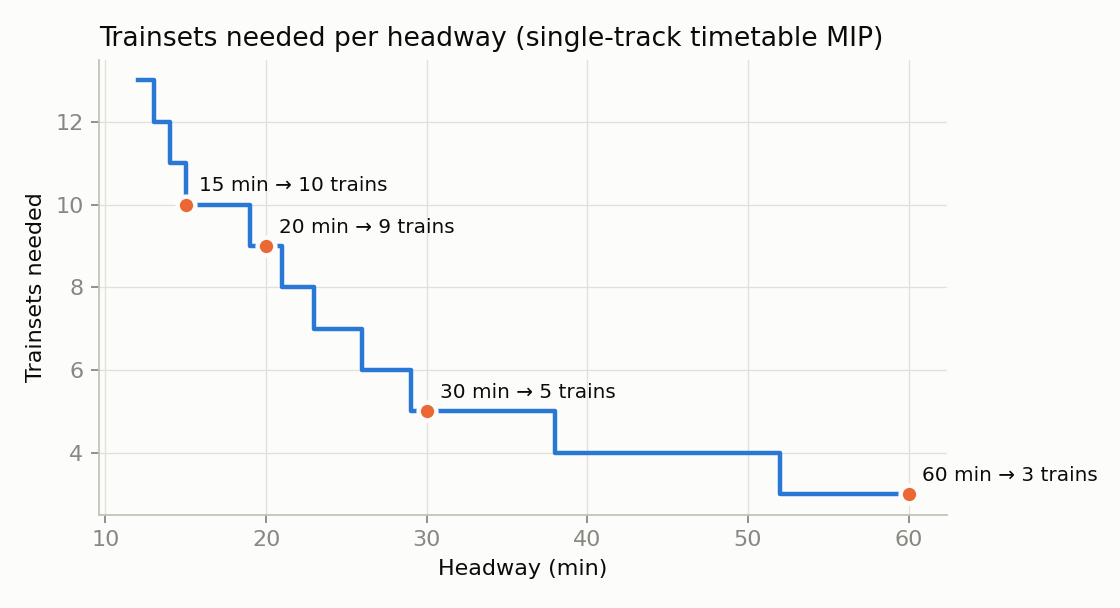
\includegraphics[width=0.72\textwidth]{fig_headway_ladder.png}
\caption{Minimum trains for each uniform headway (calibrated track, 0.5-minute buffer).}\label{fig:ladder}
\end{figure}

\subsection{The proposed timetables}
Table~\ref{tab:tt} compares NJ TRANSIT's timetable with six pattern timetables (T8--T3) and five uniform ones (U8--U4). All are printed station by station in the accompanying \emph{Timetable Book} and can be browsed on the dashboard's Timetables tab. Figures~\ref{fig:ttcompare}--\ref{fig:tttiers} compare them.

\begin{table}[ht]\centering\small
\begin{tabular}{@{}lrrrrrrrr@{}}
\toprule
Timetable & Trains & Trips & Train- & AM gap & AM gap & Midday & Avg & Meet \\
 & peak/mid & & hours & $\to$Trenton & $\to$Camden & gap & wait & conflicts \\
 & & & & mean / max & mean / max & mean & (min) & \\
\midrule
NJT current & 8/6 & 87 & 109 & 17.5 / 30 & 18.2 / 30 & 30.0 & 12.9 & 1 \\
\midrule
T8 (8 trains peak, 6 midday) & 8/6 & 88 & 109 & 18.4 / 21 & 18.8 / 24 & 26.2 & 12.9 & 0 \\
T7 (7 peak, 6 midday) & 7/6 & 80 & 99 & 21.8 / 26 & 21.3 / 30 & 25.6 & 14.0 & 0 \\
T6 (6 peak, 5 midday) & 6/5 & 69 & 86 & 25.0 / 26 & 24.7 / 31 & 28.3 & 15.5 & 0 \\
T5 (5 all day) & 5/5 & 62 & 77 & 30.2 / 31 & 30.2 / 31 & 30.0 & 16.0 & 0 \\
T4 (4 all day) & 4/4 & 48 & 60 & 37.7 / 38 & 37.5 / 38 & 37.5 & 21.1 & 0 \\
T3 (3 all day) & 3/3 & 37 & 46 & 51.5 / 52 & 46.3 / 52 & 49.7 & 27.2 & 0 \\
\midrule
U8: every 21 min peak, 30 off-peak & 8/5 & 74 & 98 & 21.0 / 21 & 20.0 / 21 & 30.0 & 14.2 & 7 \\
U7: every 23 min peak, 30 off-peak & 8/6 & 71 & 100 & 23.0 / 23 & 22.6 / 23 & 30.0 & 14.7 & 6 \\
U6: every 26 min peak, 30 off-peak & 7/6 & 66 & 96 & 26.0 / 26 & 24.7 / 26 & 30.0 & 15.7 & 4 \\
U5: every 29 min peak, 30 off-peak & 6/5 & 63 & 77 & 29.0 / 29 & 23.8 / 29 & 30.0 & 16.8 & 6 \\
U4: every 38 min peak, 38 off-peak & 4/4 & 50 & 63 & 38.0 / 38 & 38.0 / 38 & 38.0 & 19.8 & 0 \\
\bottomrule
\end{tabular}
\caption{Current and proposed weekday timetables. Gaps are measured at Walter Rand, in minutes. Average wait uses random arrivals and an assumed hourly demand profile. Conflicts are opposing trains scheduled on the same single-track section (calibrated track).}\label{tab:tt}
\end{table}

\begin{figure}[ht]\centering
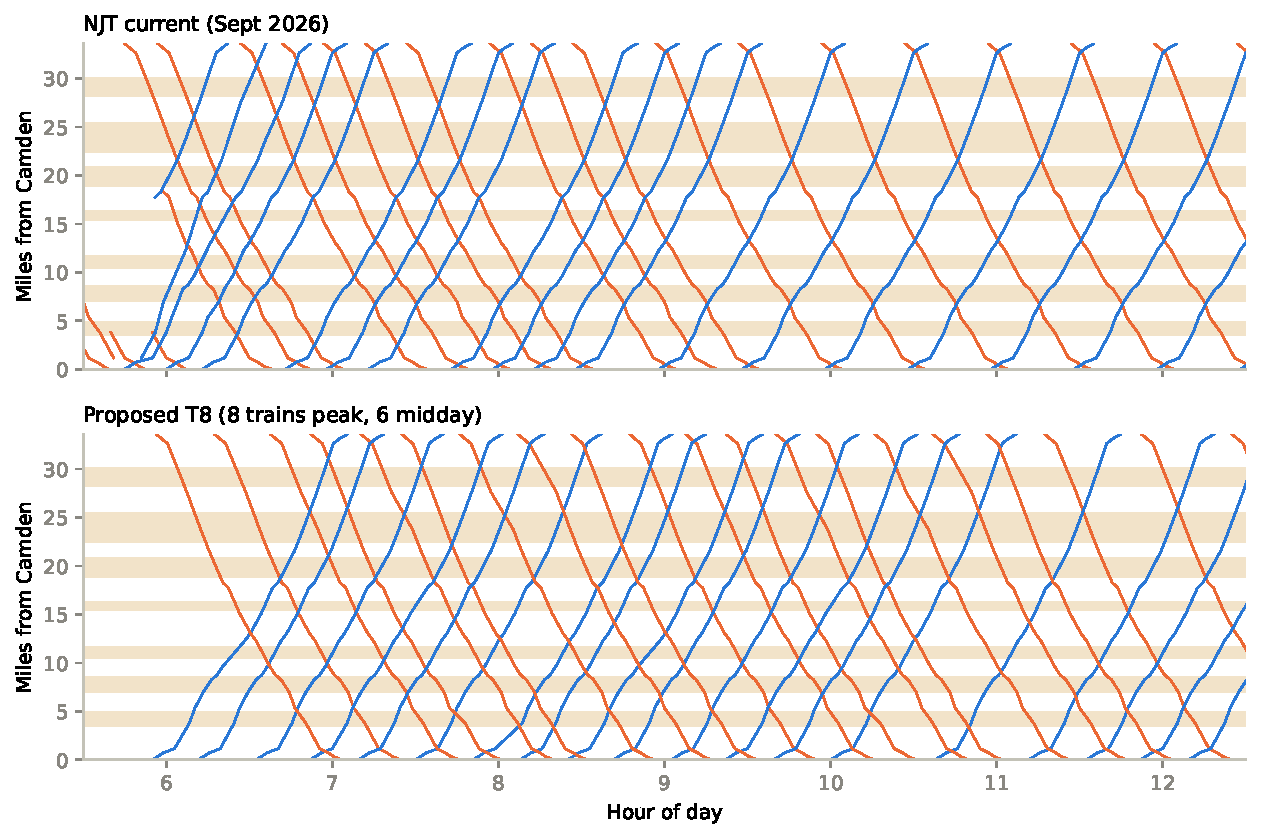
\includegraphics[width=\textwidth]{fig_tt_marey_compare.pdf}
\caption{Morning of the current timetable (top) and the proposed T8 (bottom). Same 8 trains and 150-minute cycle. T8 spreads the northbound trains 17--21 minutes apart instead of 15/15/30.}\label{fig:ttcompare}
\end{figure}
\begin{figure}[ht]\centering
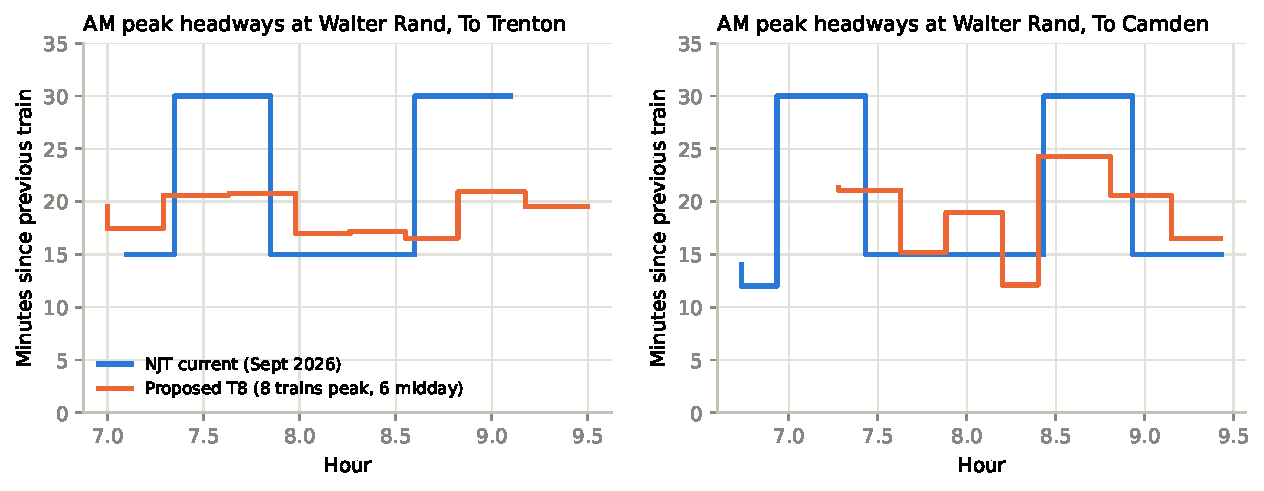
\includegraphics[width=\textwidth]{fig_tt_headways.pdf}
\caption{Morning headways at Walter Rand, current timetable vs T8.}\label{fig:tthead}
\end{figure}
\begin{figure}[ht]\centering
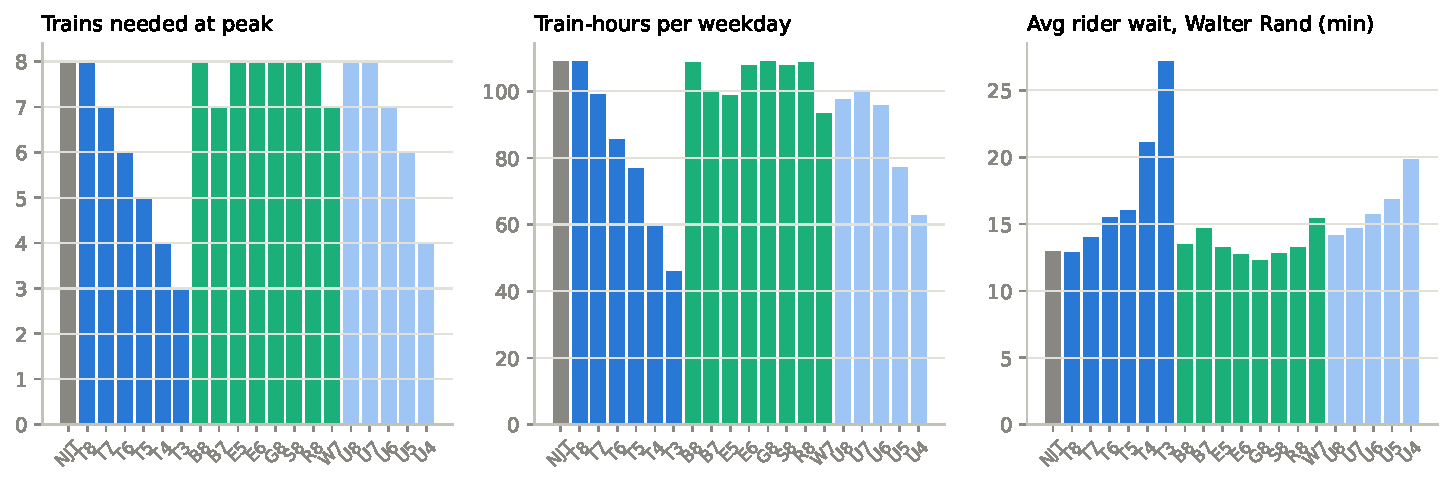
\includegraphics[width=\textwidth]{fig_tt_tiers.pdf}
\caption{Trains needed, train-hours, and average wait for each timetable. Grey: today's; blue: T8--T3; green: proposals of Section~\ref{sec:prop}; light blue: uniform timetables.}\label{fig:tttiers}
\end{figure}

\paragraph{What the comparison shows.}
\begin{itemize}
\item \textbf{T8 matches today's fleet and evens out the peaks.} It uses the same 8 peak and 6 midday trains and the same train-hours. It cuts the largest morning gap from 30 to 21 minutes toward Trenton and from 30 to 24 toward Camden. Its midday is less regular than today's 30-minute service, because the six midday trains are a subset of the peak pattern, so its all-day average wait equals today's (12.9 minutes). Its evening peak starts at 14:15 so that the returning trains also cover the 16:00--18:30 trips toward Camden. Section~\ref{sec:prop} shows that T8's tight meets cost punctuality.
\item \textbf{T7--T3 degrade gracefully.} Each needs exactly its number of trains and has no conflicts. From T5 down, service is almost perfectly even: every 30, 38 and 51 minutes.
\item \textbf{Uniform timetables are easier to remember but need retiming.} They are conflict-free within each period, but at the changeovers between peak and off-peak 4--7 pairs of trips conflict, and two of them briefly need an extra train. They are useful as targets, not yet as publishable timetables.
\end{itemize}

\clearpage
%======================================================================
\section{Proposed schedules and how they hold up to delays}\label{sec:prop}
Table~\ref{tab:tt} judges timetables as printed. This section runs them through the delay simulation of Section~\ref{sec:delaymodel}. Each proposal changes one thing, so its effect can be read off directly. All are conflict-free, in the Timetable Book, and on the dashboard's Timetables and Proposals tabs.
\begin{description}[itemsep=1pt]
\item[T8] 8 trains, peak gaps evened out; meets with 0.5-minute buffers, 5-minute layovers.
\item[B8] 8 trains on a 160-minute cycle; every meet has at least 2.5 minutes of buffer; layovers at least 9 minutes (the best of a sweep over cycle, buffer and layover, Appendix~\ref{app:sweep}).
\item[B7] The same design with 7 trains; replaces T7.
\item[E5] 8 trains at the peaks, only 5 midday (every 30 minutes): the peak and midday spacing are optimized together, and one car is free midday.
\item[E6] T8 with the 6 midday trains chosen jointly with the peak (midday gaps at most 30 minutes).
\item[G8] E6 with 2-minute meet buffers.
\item[S8] E6 with 6\% of running time moved into scheduled holds just before each single-track section.
\item[R8] 8 trains on a 160-minute cycle with 8-minute layovers but 0.5-minute buffers.
\item[W7] Summer: running times +6\% (heat speed restrictions), 7 trains on 160 minutes, 5 midday.
\end{description}
The pattern model of Section~\ref{sec:pattern} was extended for these: a subset of trains whose gaps enter the objective (the midday trains), a minimum hold before each single-track section, separate minimum layovers at each end, and a meet buffer $g$ as a parameter.

\begin{table}[ht]\centering\small
\begin{tabular}{@{}lrrrrrrrrr@{}}
\toprule
Schedule & Trains & Train- & Longest & Avg & On time & On time & Avg late- & Wait + & Held for \\
 & peak/mid & hours & AM gap & wait & normal & hot day & ness & lateness & meets \\
 & & & (min) & (min) & (\%) & (\%) & (min) & (min) & (min/day) \\
\midrule
NJT today & 8/6 & 109 & 30 & 12.9 & 84 & 60 & 2.7 & 15.7 & 234 \\
\midrule
T8 & 8/6 & 109 & 24 & 12.9 & 72 & 36 & 4.9 & 17.7 & 386 \\
\midrule
B8 & 8/6 & 109 & 31 & 13.5 & 87 & 79 & 2.2 & 15.7 & 174 \\
B7 & 7/6 & 100 & 32 & 14.6 & 89 & 79 & 1.8 & 16.5 & 127 \\
E5 & 8/5 & 99 & 28 & 13.3 & 81 & 61 & 3.2 & 16.5 & 226 \\
E6 & 8/6 & 108 & 26 & 12.7 & 73 & 41 & 4.8 & 17.5 & 357 \\
G8 & 8/6 & 109 & 29 & 12.3 & 80 & 55 & 3.4 & 15.7 & 253 \\
S8 & 8/6 & 108 & 26 & 12.8 & 74 & 43 & 4.7 & 17.5 & 328 \\
R8 & 8/6 & 109 & 26 & 13.3 & 80 & 59 & 3.5 & 16.8 & 312 \\
W7 & 7/5 & 93 & 32 & 15.4 & 92 & 86 & 1.4 & 16.8 & 127 \\
U8 & 8/5 & 98 & 21 & 14.2 & 88 & 73 & 2.0 & 16.2 & 198 \\
\bottomrule
\end{tabular}
\caption{Proposed schedules, 400 simulated weekdays each (hot day: 400 more with running times +6\%). ``Held for meets'' is the total time trains wait at single-track entrances for a late opposing train. Wait + lateness is the average scheduled wait at Walter Rand plus the average lateness at the end of the trip, a simple measure of the total rider penalty.}\label{tab:prop}
\end{table}

\begin{figure}[ht]\centering
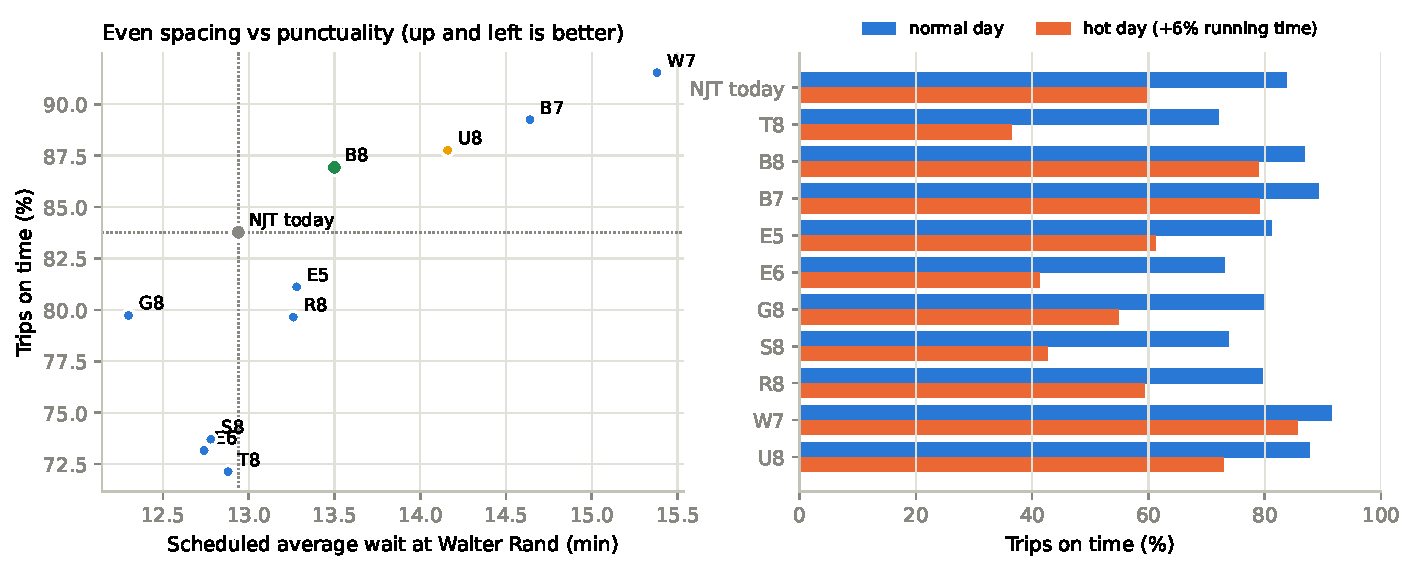
\includegraphics[width=\textwidth]{fig_prop_tradeoff.pdf}
\caption{Left: each schedule's scheduled average wait against its simulated on-time rate. Dotted lines: today's timetable. Right: on-time rates on normal and hot days.}\label{fig:proptradeoff}
\end{figure}

\paragraph{Evening out the gaps alone makes trains later.} T8 is on time 72\% of trips, against 84\% for today's timetable, and only 36\% on a hot day. Figure~\ref{fig:propwhy} shows why. In T8, 22\% of the scheduled meets have less than a minute of slack, against 7\% today, so a train that is one minute late holds the opposing train at the siding. And 79\% of T8's turnbacks are under 8 minutes, against 28\% today (median 6.1 against 9.0 minutes). NJ TRANSIT's 30-minute gap is where its recovery time lives. This is a known effect: minimizing waiting alone packs a timetable and makes it fragile \citep{fischetti2009light,liebchen2009concept}.

\begin{figure}[ht]\centering
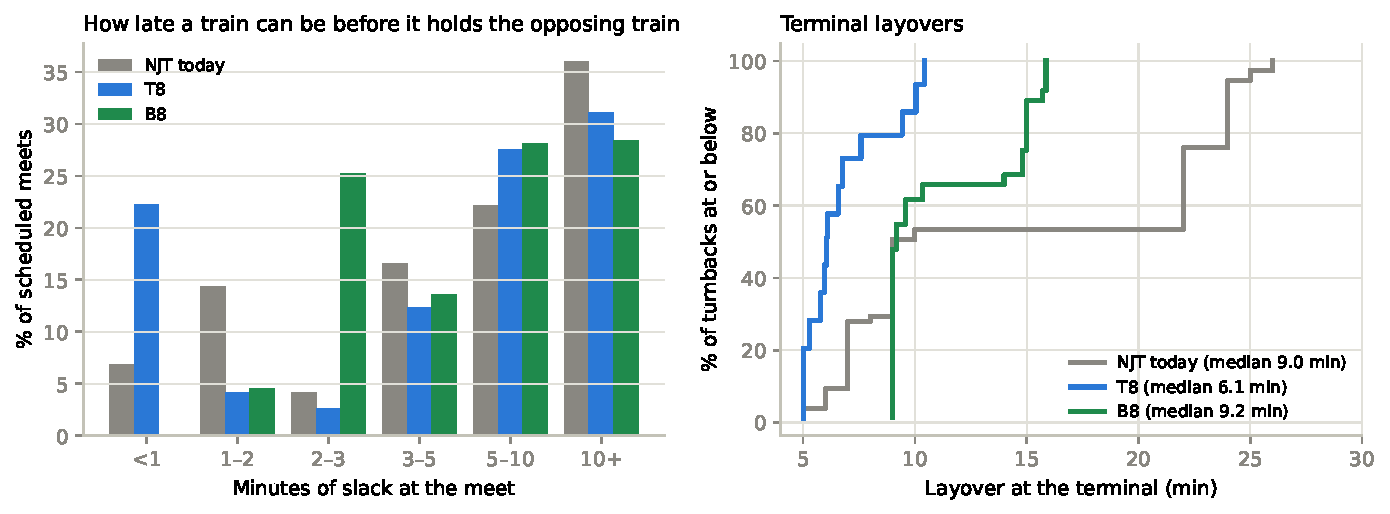
\includegraphics[width=\textwidth]{fig_prop_why.pdf}
\caption{Left: slack at scheduled single-track meets, i.e.\ how late the first train can be before it delays the opposing train. Right: distribution of terminal layovers.}\label{fig:propwhy}
\end{figure}

\paragraph{Slack at meets and at the terminals together fix it.} Longer layovers alone (R8) or meet buffers alone (G8) recover part of the loss (80\%). Moving 6\% of running time into holds before single track (S8) barely helps (74\%), because the holds sit where trains are already waiting for each other. B8 does both and is on time 87\% of trips, 79\% on a hot day. It uses the same 8 trains and 109 train-hours as today. The price is spacing: B8's longest morning gap is 31 minutes and its average wait is 13.5 minutes (today 12.9), so wait plus lateness per rider is the same as today's (15.7 minutes). With 8 trains and this track, even spacing and punctuality trade off (Figure~\ref{fig:proptradeoff}); B8 chooses punctuality. Figure~\ref{fig:propreplay} replays the same typical morning under both timetables.

\begin{figure}[ht]\centering
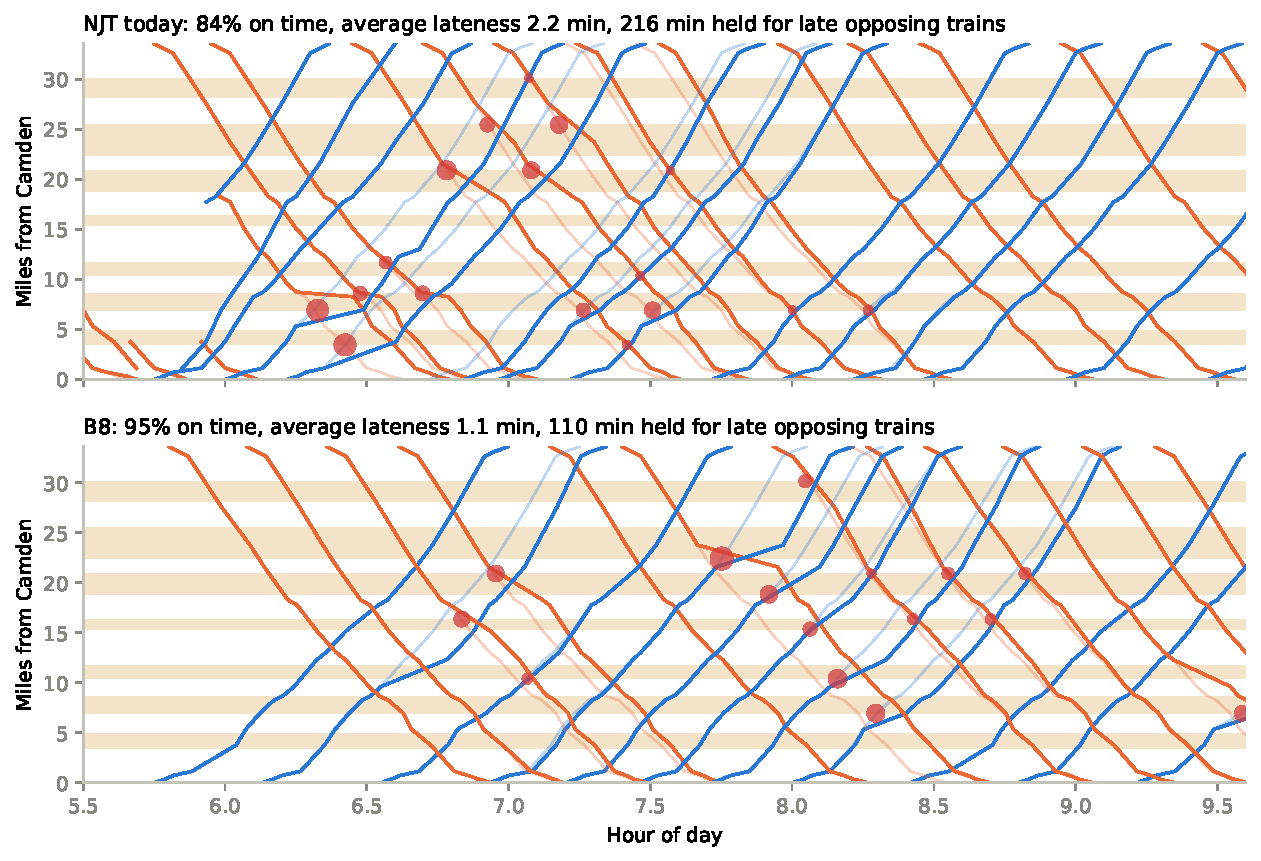
\includegraphics[width=\textwidth]{fig_prop_replay.pdf}
\caption{The same simulated morning under today's timetable (top) and B8 (bottom). Faint lines: schedule. Solid lines: simulated trains. Red dots: a train held at a single-track entrance for a late opposing train (size = minutes). Shaded: single track.}\label{fig:propreplay}
\end{figure}

\paragraph{Other findings.}
\begin{itemize}
\item \textbf{B7} (7 trains) is on time 89\%, against 76\% for T7, and should replace T7 in the playbook.
\item \textbf{W7}, the summer timetable, is on time 86\% on hot days (today's timetable: 60\%), with a longer average wait (15.4 minutes). In the fleet simulation, publishing W7 for the summer also cuts summer cancellations from 3.8\% to 2.9\% (Table~\ref{tab:propyear}), because it frees a car.
\item \textbf{E5} runs midday with 5 trains and saves 10 train-hours a day (about \$4{,}000 at \$400 per train-hour) at 81\% on time. It bears on the client question about the sixth midday train: E5 is 3 points below today's on-time rate, a rough price of the sixth train's recovery time. E5 is useful on days a car is due for maintenance.
\item \textbf{Uniform U8} does well in this simulation (88\%) because its 21-minute headway uses a 168-minute cycle with long layovers, but it still has 7 conflicts at the changeovers.
\end{itemize}

\paragraph{Robustness of the conclusion.} Figure~\ref{fig:propsens} reruns the comparison with a smaller or larger supplement, twice or half the incidents, doubled segment noise, and a 6-minute minimum turnaround. The on-time rates move by up to 25 points, but the ranking does not: B8 and B7 beat today's timetable and T8 trails it in every case.

\begin{figure}[ht]\centering
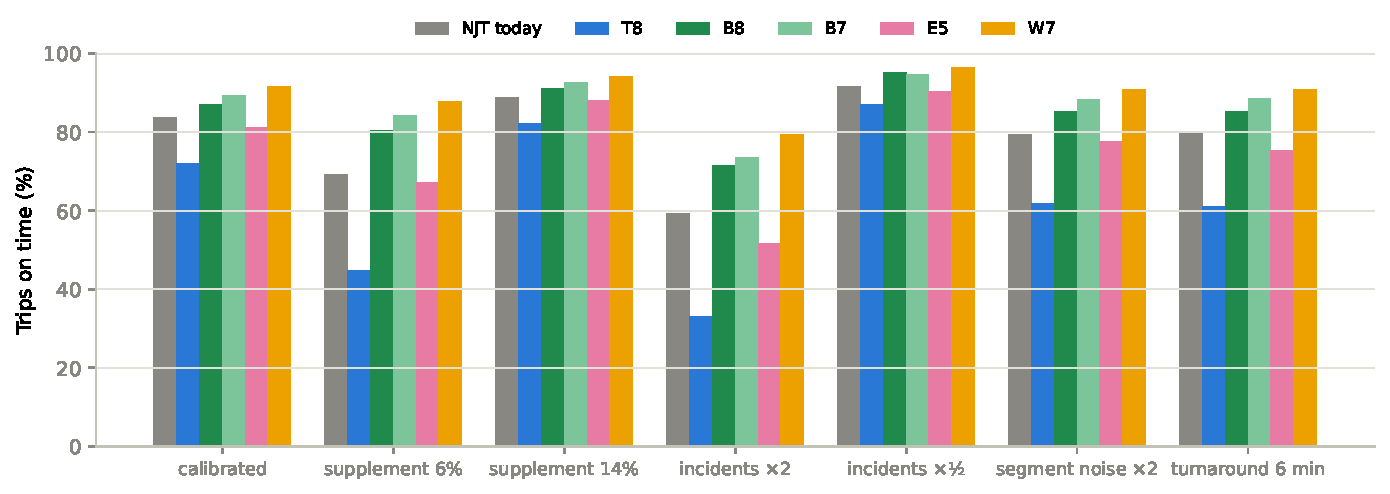
\includegraphics[width=\textwidth]{fig_prop_sens.pdf}
\caption{On-time rates under alternative delay assumptions (200 simulated days each).}\label{fig:propsens}
\end{figure}

\paragraph{Over a year.} Table~\ref{tab:propyear} runs the proposals through the fleet simulation of Section~\ref{sec:results} (breakdowns, repairs, rescues; placeholder parameters). Replacing T8/T7 by B8/B7 leaves cancellations about unchanged (2.2\% vs 2.3\%), so the punctuality gain is free. Adding the summer timetable brings annual cancellations to 2.0\% and summer cancellations to 2.9\%.

\begin{table}[ht]\centering\small
\begin{tabular}{@{}lrrrrr@{}}
\toprule
Plan & Cancelled & Summer & Winter & Avg wait & Operating \\
 & (\%) & (\%) & (\%) & (min) & (\$k/day) \\
\midrule
NJT published, no protect & 11.8 & 21.5 & 12.8 & 17.8 & 39.1 \\
Tiers T8--T3, 1 protect & 2.3 & 3.4 & 2.7 & 16.9 & 36.8 \\
Robust tiers B8/B7/T6--T3, 1 protect & 2.2 & 3.8 & 2.3 & 17.2 & 37.8 \\
Robust tiers + summer W7, 1 protect & 2.0 & 2.9 & 2.3 & 17.1 & 37.8 \\
E5 on 8-car days, B7/T6--T3, 1 protect & 2.2 & 3.5 & 2.3 & 17.2 & 35.6 \\
Robust tiers B8/B7/T6--T3, 0 protect & 4.2 & 7.3 & 4.5 & 17.2 & 38.7 \\
\bottomrule
\end{tabular}
\caption{Ten simulated years per plan (dashboard engine). ``Robust tiers'' use B8 with 8 trains, B7 with 7, and T6--T3 below. The wait includes cancelled trips but not lateness.}\label{tab:propyear}
\end{table}

\paragraph{Recommended package.}
\begin{enumerate}
\item Weekday base timetable B8 (8 trains), with B7 for 7-car days and T6--T3 below, chosen at the 6\,am hold sheet with one protect car.
\item A published summer timetable (W7) for June--August.
\item E5 on days when a car must go to the shop midday.
\end{enumerate}
Before any of this goes to NJ TRANSIT, the delay model must be checked against train-level arrival records (Data Request priority 1) and the siding positions against the official track chart.

\clearpage
%======================================================================
\section{Putting it together: one measure, calibrated inputs, validation}\label{sec:combined}
Sections~\ref{sec:prop} and \ref{sec:results} use two separate simulations. The fleet simulation counts cancellations from breakdowns and car shortages. The delay simulation counts lateness when every trip runs. This section joins them and replaces the placeholder inputs with values taken from data.

\subsection{How the two simulations are combined}
For each simulated day, the fleet simulation (the dashboard engine) draws the cars available at 6\,am, chooses the day's timetable by the policy, and simulates breakdowns, rescues, and cancellations. The trip-miles that run are then weighted by the delay-simulation on-time probability for that timetable: the normal-day value, or in summer a mix with 23\% hot days. Trenton averages 21 days at or above 90\textdegree F each summer (Section~\ref{sec:data}). Dividing by the trip-miles in today's timetable gives the day's RTD. We average over 10 simulated years of 365 days after a 60-day warm-up, and the range across the 10 years is reported.

\subsection{Inputs taken from data}
\begin{itemize}
\item \textbf{Miles between failures.} NJ TRANSIT's monthly River LINE series \citep{njt_mdbf} averages 3{,}661 miles in 2024--25 and 3{,}568 miles in March--August 2026. Its 2022 and 2024 annual means (22{,}337 and 4{,}192) match the figures reported in the press, so the press numbers come from this series.
\item \textbf{Cost per train-hour: \$547.} This is NTD FY2024 vehicle operations plus vehicle maintenance (\$20.9 million) divided by 38{,}212 vehicle revenue hours \citep{ntd_ts21}. It excludes administration and non-vehicle maintenance, which do not vary with service. The earlier \$400 was a placeholder; the full average is \$952.
\item \textbf{Delay regimes.} The delay simulation's incident rate is fitted to 83\% on time for the Alstom era \citep{news12_2025,njtod2026} and to 93\% for 2026 \citep{ols2027njt}.
\item \textbf{Repair times.} There are no public repair records, so repair times are inferred from fleet behavior:
  \begin{itemize}
  \item \emph{2024--25: 10 days.} This makes summer availability too low for the 8-train timetable on most days. NJ TRANSIT did in fact move to a 30-minute interim schedule with buses in August 2024 \citep{njt2024interim}.
  \item \emph{2026: 5 days.} This gives about 12 cars on a typical day. NTD reports 12 vehicles in maximum service in March--June 2026 \citep{ntd_monthly}.
  \item Both are varied in Table~\ref{tab:rtdsens}.
  \end{itemize}
\end{itemize}
The three scenarios are:
\begin{itemize}
\item \textbf{S1, Alstom era 2024--25:} MDBF 3{,}661, 10-day repairs, 83\% delay regime.
\item \textbf{S2, NJ TRANSIT 2026:} MDBF 3{,}568, 5-day repairs, 93\% regime.
\item \textbf{S3, renewed fleet:} MDBF 10{,}000 (about the 2017 level), 5-day repairs, 93\% regime.
\end{itemize}

\subsection{Validation against 2024--26 evidence}
Table~\ref{tab:valid} compares the model with everything we can observe. Items marked \emph{fitted} were used to set inputs and do not test the model. Items marked \emph{tested} were not used.
{\small
\begin{longtable}{@{}p{3.5cm}p{4.2cm}p{4.2cm}p{3.1cm}@{}}
\caption{Model against observed data.}\label{tab:valid}\\
\toprule
Evidence & Observed & Model & Verdict \\ \midrule\endfirsthead
\toprule Evidence & Observed & Model & Verdict \\ \midrule\endhead
Miles between failures & NJ TRANSIT series: 3{,}661 (2024--25), 3{,}568 (2026) \citep{njt_mdbf} & Input & Fitted \\
In-service failures per year & 267 major (435 total), NTD FY2024 \citep{ntd_breakdowns2224} & S1: 0.79 per day, about 290 a year & Tested: close (+8\%) \\
On-time share of trips run, 2024--25 & 84\% (2025) \citep{njtod2026}; about 87\% (2024--25) \citep{ols2027njt}; 82.3\% (July 2025) \citep{news12_2025} & S1, today's timetable: 82\% (all year, including heat and blockages) & Tested: 2--5 points low \\
Worst days & 45\% (summer 2024), 56\% (summer 2025) \citep{ols2027njt} & Expected worst weekday of a summer: 20\% with the hot-day model; 40\% without & Tested: too harsh. The +6\% all-day heat assumption overstates bad days \\
Summer car shortage, 2024 & NJ TRANSIT cut to a 30-minute interim schedule with buses (August 2024) \citep{njt2024interim} & S1: 7.2 cars on an average summer day; fewer than 8 on 59\% of summer days & Tested: consistent \\
Cars in service, 2026 & NTD vehicles in maximum service: 12 (March--June), 8 (July) \citep{ntd_monthly} & S2: 12.7 cars on average; at least 12 on 72\% of days (56\% in summer) & Tested: consistent \\
On time after the takeover & ``above 93 percent'' \citep{ols2027njt} & 93\% & Fitted \\
Cancellations & 15 cancelled trips in July 2025 \citep{singleton2025} & S1, today's timetable: 9.7\% of trips (hundreds a month in summer) & Not resolved: either shortages are overstated or a reduced timetable was in force; cancellation records needed \\
Ridership response & +22\% (June) and +12\% (July 2026) year over year \citep{ntd_monthly} & Not modeled & Gap \\
\bottomrule
\end{longtable}}
The model reproduces failure counts and the direction and timing of the fleet crisis and recovery. It is somewhat pessimistic about punctuality, and clearly too pessimistic about the worst (hot) days. It cannot yet be checked on cancellations, the quantity Q3 depends on.

\subsection{Results}
\begin{table}[ht]\centering\small
\begin{tabular}{@{}lccccccc@{}}
\toprule
& \multicolumn{3}{c}{RTD, \% (range over 10 years)} & Cancelled \% & On time \% of & Cost \\
Policy & S1 2024--25 & S2 2026 & S3 renewed & S1 / S2 & trips run, S1 / S2 & \$k/day, S2 \\
\midrule
Today's timetable & 69.4 (68--71) & 84.2 (84--85) & 85.8 (86--86) & 9.7 / 2.0 & 82 / 92 & 59.4 \\
B8 every day & 73.4 (71--77) & 87.5 (87--88) & 89.5 (89--90) & 12.1 / 2.4 & 87 / 94 & 59.1 \\
Tiers T8--T3 (+1 protect) & 65.4 (64--67) & 83.3 (83--84) & 84.7 (85--85) & 2.2 / 2.0 & 74 / 86 & 59.1 \\
Robust tiers (+1 protect) & 74.4 (73--76) & 87.5 (87--88) & 89.5 (89--90) & 2.4 / 1.9 & 87 / 94 & 59.1 \\
Robust tiers + summer W7 & 73.5 (71--76) & 85.2 (85--85) & 86.8 (87--87) & 2.3 / 1.8 & 87 / 94 & 57.2 \\
Robust tiers (no protect) & 75.3 (72--78) & 87.5 (87--88) & 89.5 (89--90) & 4.0 / 2.2 & 87 / 94 & 59.1 \\
\bottomrule
\end{tabular}
\caption{Headline results. Cost is train-hours $\times$ \$547. All policies except ``today'' and ``B8 every day'' choose the timetable from the 6\,am car count.}\label{tab:rtd}
\end{table}

\begin{figure}[ht]\centering
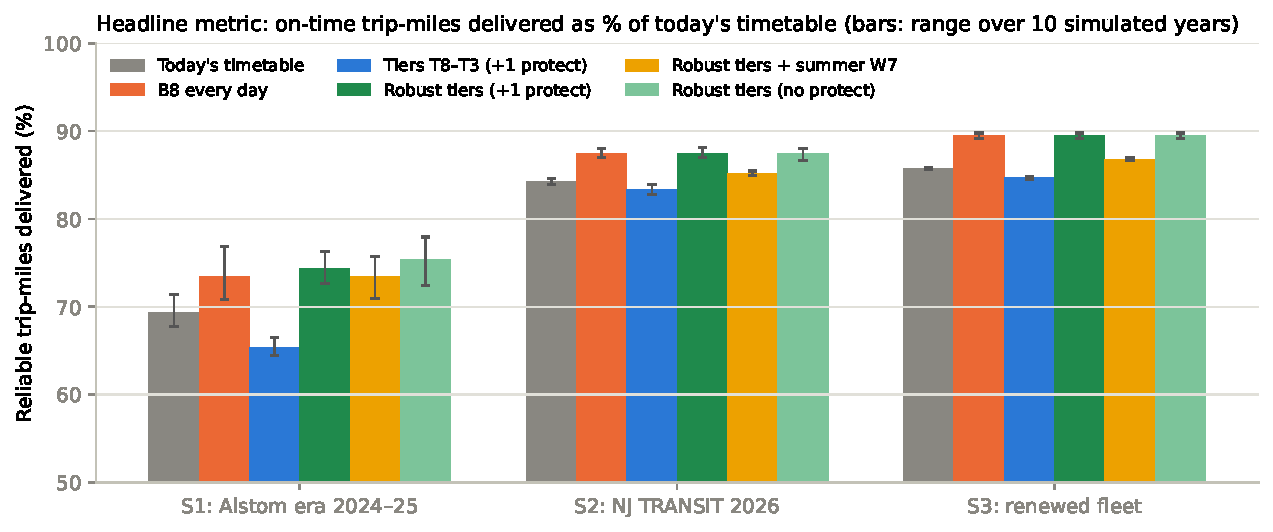
\includegraphics[width=\textwidth]{fig_rtd.pdf}
\caption{Headline measure by scenario and policy. The vertical axis starts at 50\%.}\label{fig:rtd}
\end{figure}
\begin{figure}[ht]\centering
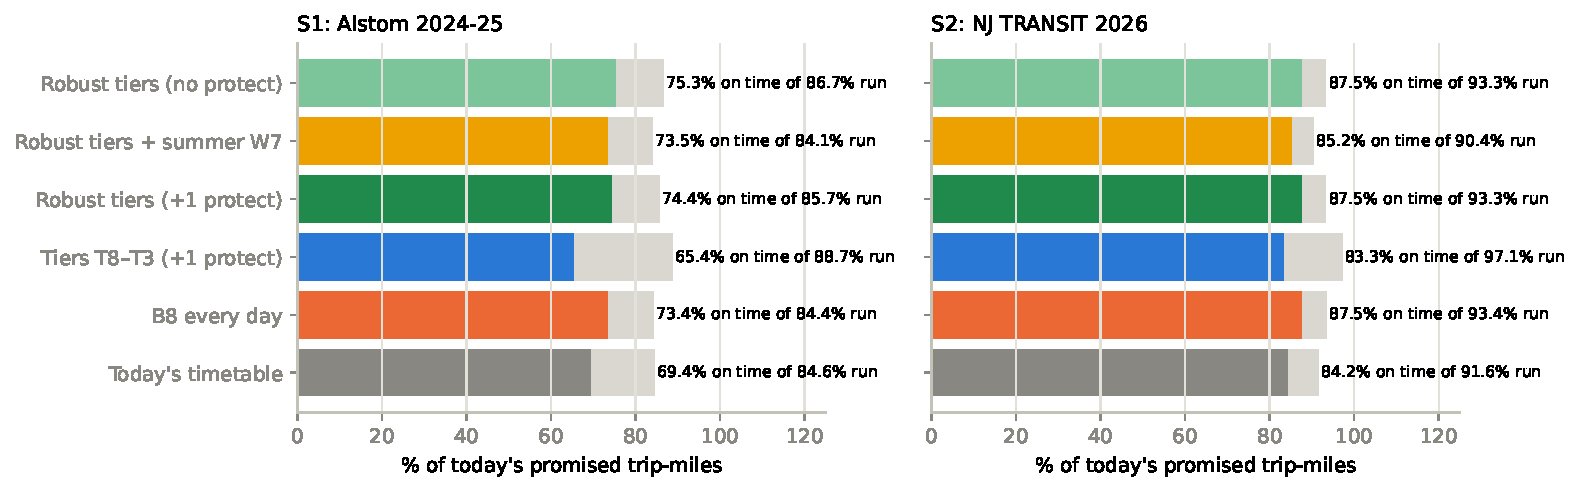
\includegraphics[width=\textwidth]{fig_rtd_decomp.pdf}
\caption{Trip-miles run (grey) and the part of them on time (colored), as a percentage of today's timetable, in S1 and S2.}\label{fig:rtddecomp}
\end{figure}

\paragraph{What the combined measure shows.}
\begin{enumerate}
\item \textbf{Fleet reliability matters most.} Going from S1 to S2 raises RTD by 13--18 points for every policy. More than half of this comes from fewer delays; the rest from fewer cancellations. The 2026 maintenance and operations changes are worth more than any timetable.
\item \textbf{B8 is the best single change.} It adds 3--4 points over today's timetable in every scenario at the same train-hours and cost (Figure~\ref{fig:rtd}).
\item \textbf{Choosing the timetable each morning helps only when cars are short.} In S1, robust tiers raise RTD to 74.4\% against 73.4\% for B8 every day, and cut cancellations from 12.1\% to 2.4\%. In S2 and S3 the car count rarely drops below 9, so tiering and B8 every day give the same result. Tiering remains insurance for the next fleet crisis.
\item \textbf{The T8--T3 tiers of revision 2 are not recommended.} T8 and T7 are too fragile (Section~\ref{sec:prop}), so the tiers score below today's timetable on RTD in every scenario despite cancelling least. Counting cancellations alone would have hidden this.
\item \textbf{The summer timetable W7 is not supported on this measure.} It cuts trips to buy punctuality, and it loses about 1 point of RTD in S1 and 2--3 points in S2 and S3 against robust tiers. The hot-day effect it guards against is overstated in our model (Table~\ref{tab:valid}). It stays an option only if NJ TRANSIT confirms long heat speed restrictions.
\item \textbf{A protect car costs a little RTD but prevents surprises.} Without it, cancellations rise from 2.4\% to 4.0\% in S1 while RTD edges up. RTD does not distinguish planned reductions from unplanned cancellations, which riders value differently \citep{usdot2016vtts}. We keep the protect car.
\end{enumerate}

\begin{table}[ht]\centering\small
\begin{tabular}{@{}lccccccc@{}}
\toprule
Scenario variant & Mean cars & Today & B8 every day & Tiers T8--T3 & Robust tiers & + summer W7 & Robust, no protect \\
\midrule
S1, repairs 8 days & 10.3 & 72.4 & 77.9 & 66.8 & 77.8 & 76.4 & 78.4 \\
S1 (repairs 10 days) & 8.9 & 69.4 & 73.4 & 65.4 & 74.4 & 73.5 & 75.3 \\
S1, repairs 12 days & 7.5 & 63.0 & 68.9 & 63.1 & 68.7 & 68.9 & 70.1 \\
S2, repairs 3 days & 14.7 & 84.6 & 88.0 & 83.9 & 88.0 & 85.4 & 88.0 \\
S2 (repairs 5 days, MDBF 3,568) & 12.7 & 84.2 & 87.5 & 83.3 & 87.5 & 85.2 & 87.5 \\
S2, repairs 8 days & 9.9 & 80.0 & 83.9 & 79.8 & 83.3 & 82.3 & 84.2 \\
S2, MDBF 2,500 & 11.5 & 82.1 & 85.1 & 81.7 & 84.8 & 83.4 & 85.2 \\
\bottomrule
\end{tabular}
\caption{RTD (\%) under alternative repair times and failure rates.}\label{tab:rtdsens}
\end{table}


\paragraph{Updated playbook (S2, summer).} For each car count at 6\,am, Table~\ref{tab:pb4} gives the plan with the highest RTD among those that cancel at most 5\% of their own trips without warning. This guardrail keeps unplanned cancellations, which riders dislike more than planned reductions, in check. With 9 or more cars, run B8. With 4--8 cars, publish the matching robust tier (B7, T6, T5, T4, T3) and hold one protect car. With 3 cars, run T3 without a protect car; no plan meets the guardrail there. The dashboard's Playbook tab shows the same table for both seasons.

On days with 4--7 cars, the recommended tier delivers about the same RTD as running today's timetable with the cars available, sometimes 1--2 points less. But it cancels only about 4\% of its trips, against 15--52\%. The gain on short days is predictability: riders can rely on a published, smaller timetable instead of an unannounced one with holes. RTD alone does not capture that, which is why the guardrail is needed. If NJ TRANSIT agrees on a value for unplanned cancellations, it can replace the guardrail.
\begin{table}[ht]\centering\small
\begin{tabular}{@{}rllrrrr@{}}
\toprule
Cars & Policy & Timetable & RTD \% & RTD today's tt. \% & Cancelled \% & Today's tt. cancelled \% \\
\midrule
3 & Robust tiers, 0 protect & T3 & 37 & 30 & 10.2 & 64.7 \\
4 & Robust tiers, 1 protect & T3 & 39 & 41 & 4.1 & 52.1 \\
5 & Robust tiers, 1 protect & T4 & 49 & 51 & 3.6 & 40.2 \\
6 & Robust tiers, 1 protect & T5 & 63 & 63 & 4.8 & 26.0 \\
7 & Robust tiers, 1 protect & T6 & 70 & 72 & 4.3 & 15.0 \\
8 & Robust tiers, 1 protect & B7 & 79 & 78 & 4.4 & 7.9 \\
9 & B8 every day & B8 & 86 & 81 & 4.5 & 4.2 \\
10 & B8 every day & B8 & 87 & 82 & 3.1 & 2.7 \\
11 & B8 every day & B8 & 87 & 82 & 2.8 & 2.6 \\
12 & B8 every day & B8 & 87 & 83 & 2.5 & 2.3 \\
\bottomrule
\end{tabular}
\caption{Playbook under scenario S2, summer, 300 simulated days per row. ``Today's tt.'' is NJ TRANSIT's published timetable run with the same cars.}\label{tab:pb4}
\end{table}

\paragraph{Sensitivity.} The ranking is stable across repair times of 3--12 days and a failure interval of 2{,}500 miles (Table~\ref{tab:rtdsens}): B8 or robust tiers first, today's timetable next, T tiers last. The size of the tiering benefit depends on repair times, which only the hold sheets can settle.

\clearpage
%======================================================================
\section{Operating the timetables when cars are short}\label{sec:results}
\begin{keybox}{Note on this section}
This section uses the placeholder fleet inputs of revision 2: 4{,}192 miles between failures, 12-day repairs, and \$400 per train-hour. These are close to scenario S1, and the counts here are cancellations only. Where the two differ, Section~\ref{sec:combined} governs.
\end{keybox}
\subsection{A simulated year}
Figure~\ref{fig:year} and Table~\ref{tab:annual} compare five policies over ten simulated years:
\begin{itemize}
\item publish NJ TRANSIT's timetable and cancel what cannot run;
\item publish the proposed timetable that fits the cars, with 0 or 1 protect car;
\item publish a uniform tier, with 1 protect car.
\end{itemize}
Today's approach cancels 11.8\% of trips, 21.5\% in summer. The proposed tiers with one protect car cancel 2.3\% (3.4\% in summer). The uniform tiers do about as well on cancellations and better on waiting, but they are not yet conflict-free at changeovers, so the simulation flatters them.

\begin{table}[ht]\centering\small
\begin{tabular}{@{}lrrrrrr@{}}
\toprule
Policy & Cars avail. & Cancelled & On time & Avg wait & Operating & Rider time \\
 & (mean) & (\%) & (\%) & (min) & (\$/day) & (\$/day) \\
\midrule
NJT published, cancel what cannot run & 8.4 & 11.8 & 82.8 & 17.8 & 39{,}100 & 50{,}400 \\
Proposed tiers, 0 protect & 8.1 & 4.5 & 89.6 & 16.8 & 38{,}200 & 44{,}000 \\
Proposed tiers, 1 protect & 8.2 & \textbf{2.3} & 91.6 & 16.9 & 36{,}800 & 43{,}600 \\
Uniform tiers (flexible), 1 protect$^\ast$ & 8.5 & 2.2 & 91.9 & 14.3 & 38{,}200 & 37{,}100 \\
Uniform tiers (clock-face), 1 protect$^\ast$ & 8.9 & 1.8 & 92.2 & 15.3 & 36{,}400 & 39{,}500 \\
\bottomrule
\end{tabular}
\caption{Ten simulated years (placeholder failure parameters). ``On time'' here counts only blockage delays; Section~\ref{sec:prop} has the delay-propagation results. $^\ast$Changeovers between peak and off-peak not yet conflict-free.}\label{tab:annual}
\end{table}

\begin{figure}[ht]\centering
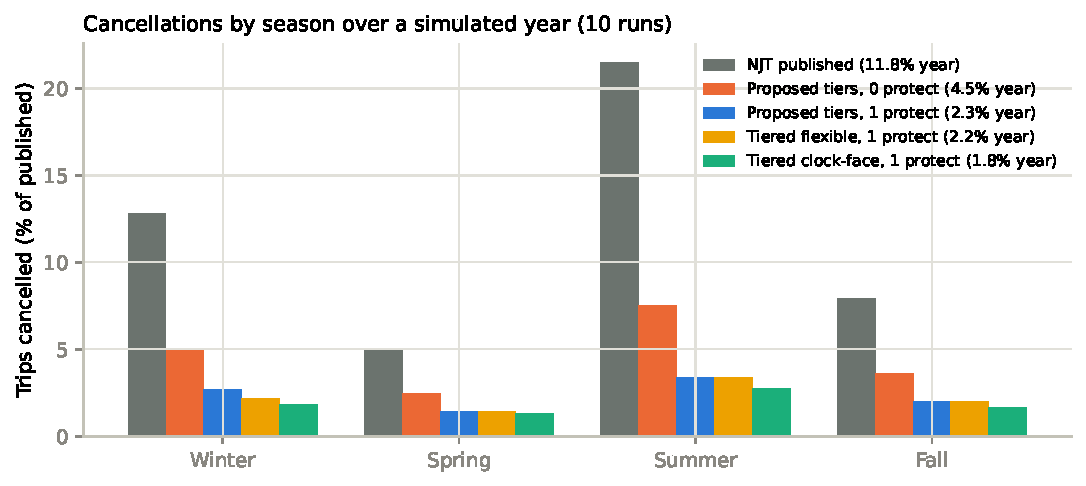
\includegraphics[width=0.85\textwidth]{fig_js_year.pdf}
\caption{Cancellations by season and policy.}\label{fig:year}
\end{figure}

\paragraph{Why summer?} The seasonal failure factors follow the client's account (heat is hardest on the hydraulics) and the literature \citep{ferranti2016heat}. Trenton averages 21 days at or above 90\textdegree F per summer, and 2024 had 27 (Figure~\ref{fig:weather}). That was the summer NJ TRANSIT cut service \citep{news12_2024}.

\begin{figure}[ht]\centering
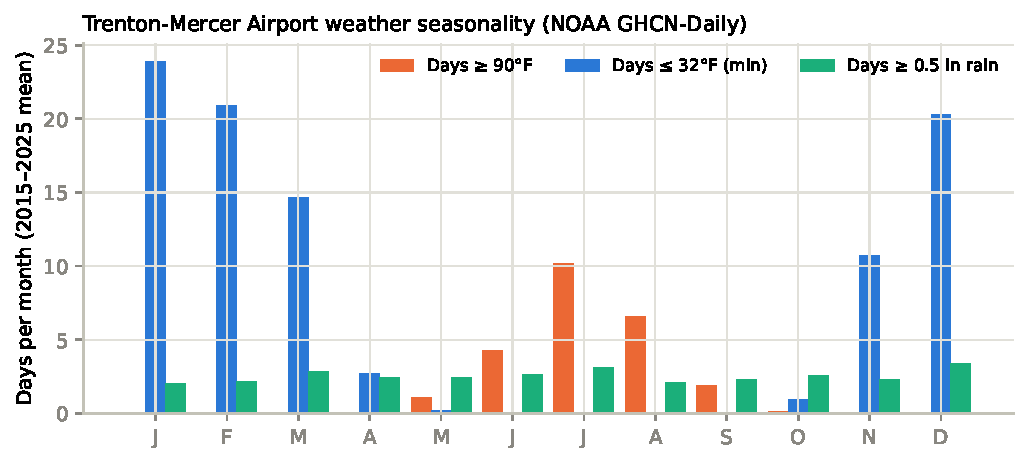
\includegraphics[width=0.78\textwidth]{fig_weather_seasonality.pdf}
\caption{Weather seasonality at Trenton-Mercer Airport, 2015--2025 \citep{noaa_ghcnd}.}\label{fig:weather}
\end{figure}

\subsection{The playbook}\label{sec:playbook}
For each morning car count, we simulated 300 days per policy (Figure~\ref{fig:playbook}) and recommend the conflict-free timetable with the lowest combined operating and rider-time cost (Table~\ref{tab:playbook}).

\begin{figure}[ht]\centering
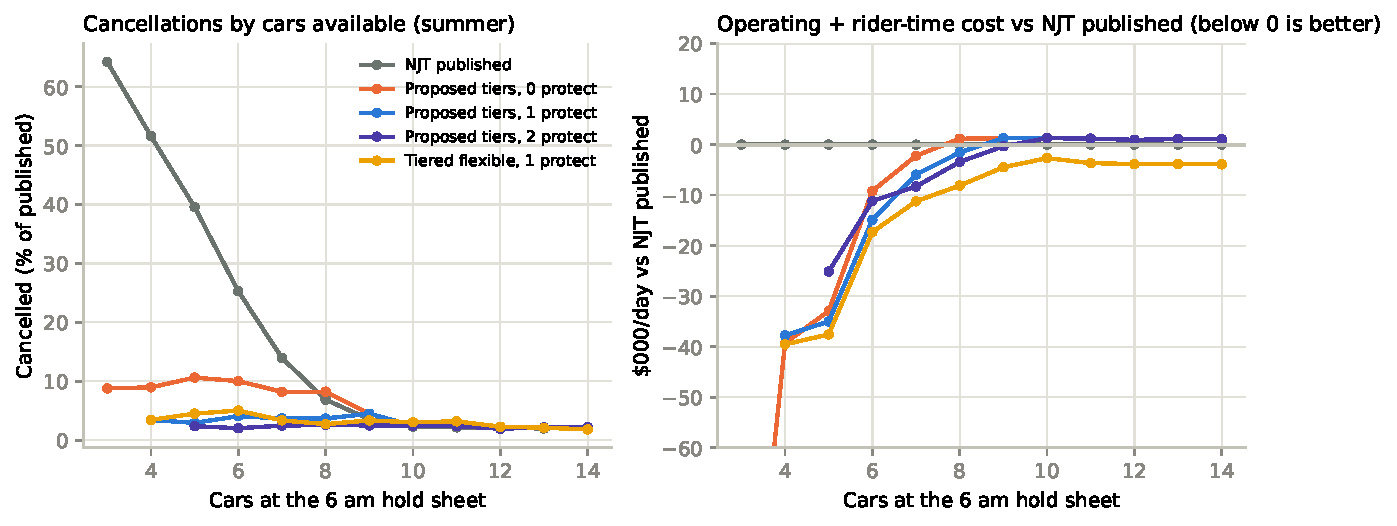
\includegraphics[width=\textwidth]{fig_js_playbook.pdf}
\caption{Cancellations (left) and daily cost relative to running NJ TRANSIT's published timetable (right), by cars available at 6\,am, summer parameters.}\label{fig:playbook}
\end{figure}

\begin{table}[ht]\centering\small
\begin{tabularx}{\textwidth}{@{}p{2cm}Lp{4.6cm}@{}}
\toprule
Cars at 6\,am & Recommended timetable (summer) & NJT published run with the cars available \\
\midrule
10 or more & Keep today's timetable, or B8 for better punctuality (Section~\ref{sec:prop}); extra cars are protect cars. & 2.0--2.3\% cancelled \\
7--9 & The tier two below the car count (T5, T6, or B7 in place of T7), holding 2 protect cars: 2.5--2.6\% cancelled. & 3.5--13.9\% cancelled \\
5--6 & T4 with 1--2 protect cars: 2.0--2.9\% cancelled. & 25--40\% cancelled \\
3--4 & T3 with 1 protect car (4 cars, 3.4\%) or T3 alone (3 cars, about 9\%); plan supplemental buses. & 52--64\% cancelled \\
\bottomrule
\end{tabularx}
\caption{Playbook (dashboard engine; \$400/train-hour; USDOT value of time).}\label{tab:playbook}
\end{table}

\subsection{Sensitivity}
Figure~\ref{fig:sens} varies the most uncertain inputs. The advantage of the proposed tiers is large when cars are often short: 4\% against 30\% cancelled when breakdowns come every 2{,}500 miles, and 2\% against 33\% when repairs take 20 days. It disappears when the fleet is reliable: with one breakdown per 8{,}000 miles or 6-day repairs, today's timetable cancels under 2\%. Where the protect car waits (Camden, Burlington, Trenton, or split between the ends) changes annual cancellations by only 0.1--0.3 points in this engine.

\begin{figure}[ht]\centering
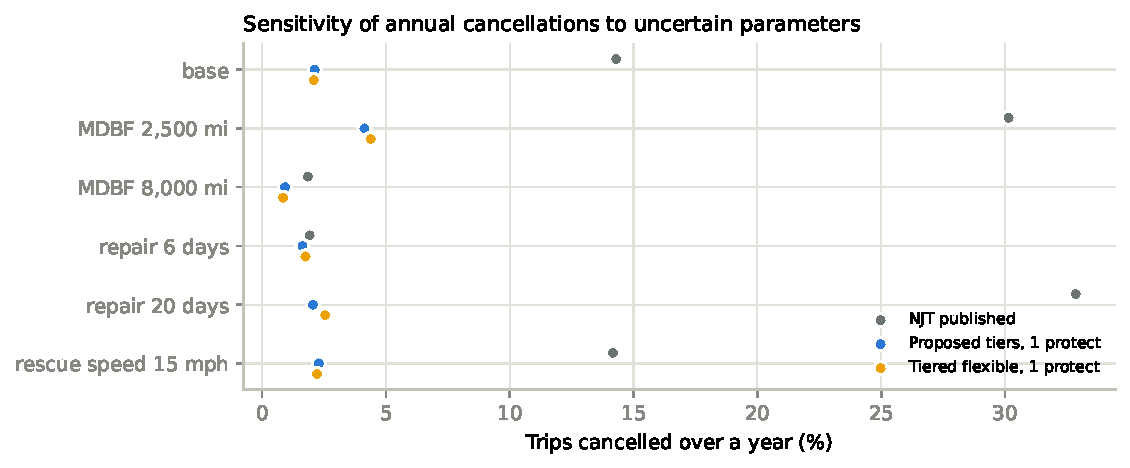
\includegraphics[width=0.8\textwidth]{fig_js_sensitivity.pdf}
\caption{Annual cancellations under alternative assumptions (8 simulated years each).}\label{fig:sens}
\end{figure}

%======================================================================
\section{The dashboard}\label{sec:dashboard}
The dashboard has eight tabs:
\begin{enumerate}
\item \textbf{Live day.} An animated map of one simulated weekday on the real track. The user can choose NJ TRANSIT's timetable, the proposed tiers, or the uniform tiers, and can break any train to watch the rescue.
\item \textbf{Timetables.} All timetables of Table~\ref{tab:tt}, with a time--distance chart and printable station-by-station grids.
\item \textbf{Proposals.} The comparison of Table~\ref{tab:prop}, the trade-off chart, a side-by-side replay of a typical, bad or hot simulated day under any two timetables (Figure~\ref{fig:dashprop}), the meet-slack chart, and the year-long results.
\item \textbf{Playbook.} What to run for each morning car count, ranked on reliable trip-miles delivered with a 5\% cancellation guardrail (Table~\ref{tab:pb4}).
\item \textbf{Policy lab.} A year-long simulation with editable assumptions and the three calibrated scenarios S1--S3; it reports the headline measure for each policy.
\item \textbf{Costs and impacts.} The day's cost account.
\item \textbf{Public data.} The charts of Section~\ref{sec:data}.
\item \textbf{About.} Assumptions and sources.
\end{enumerate}
The numbers in Sections~\ref{sec:tt}--\ref{sec:results} were produced by running the dashboard's own engine headlessly, so the report and the dashboard agree.

\begin{figure}[ht]\centering
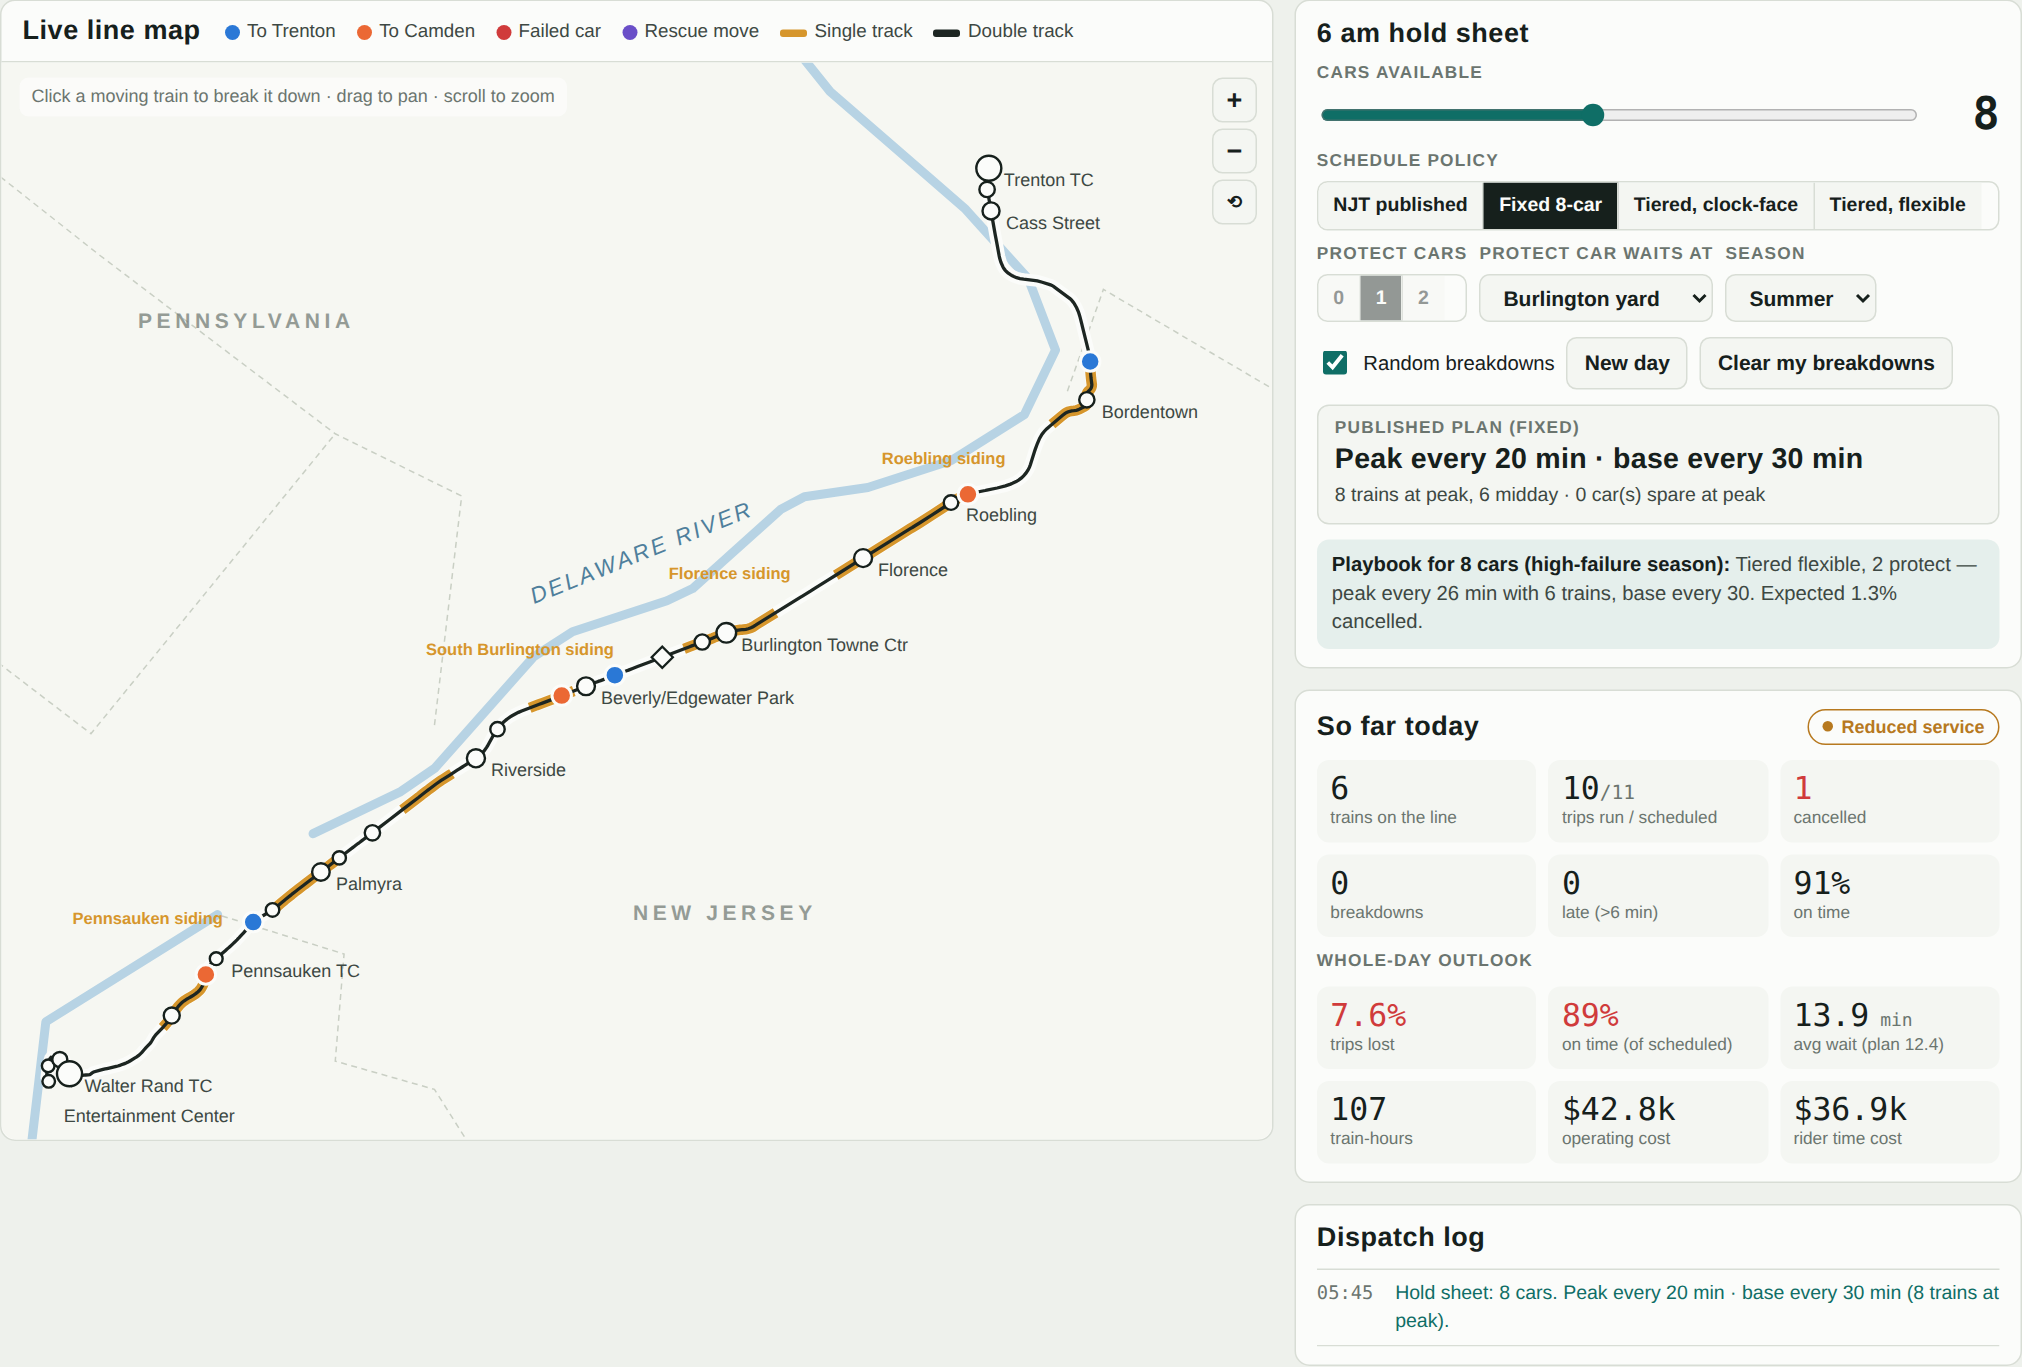
\includegraphics[width=\textwidth]{dash_live.png}
\caption{Dashboard, Live day tab: a breakdown blocks single track while a protect car heads to the failed car.}\label{fig:dash}
\end{figure}
\begin{figure}[ht]\centering
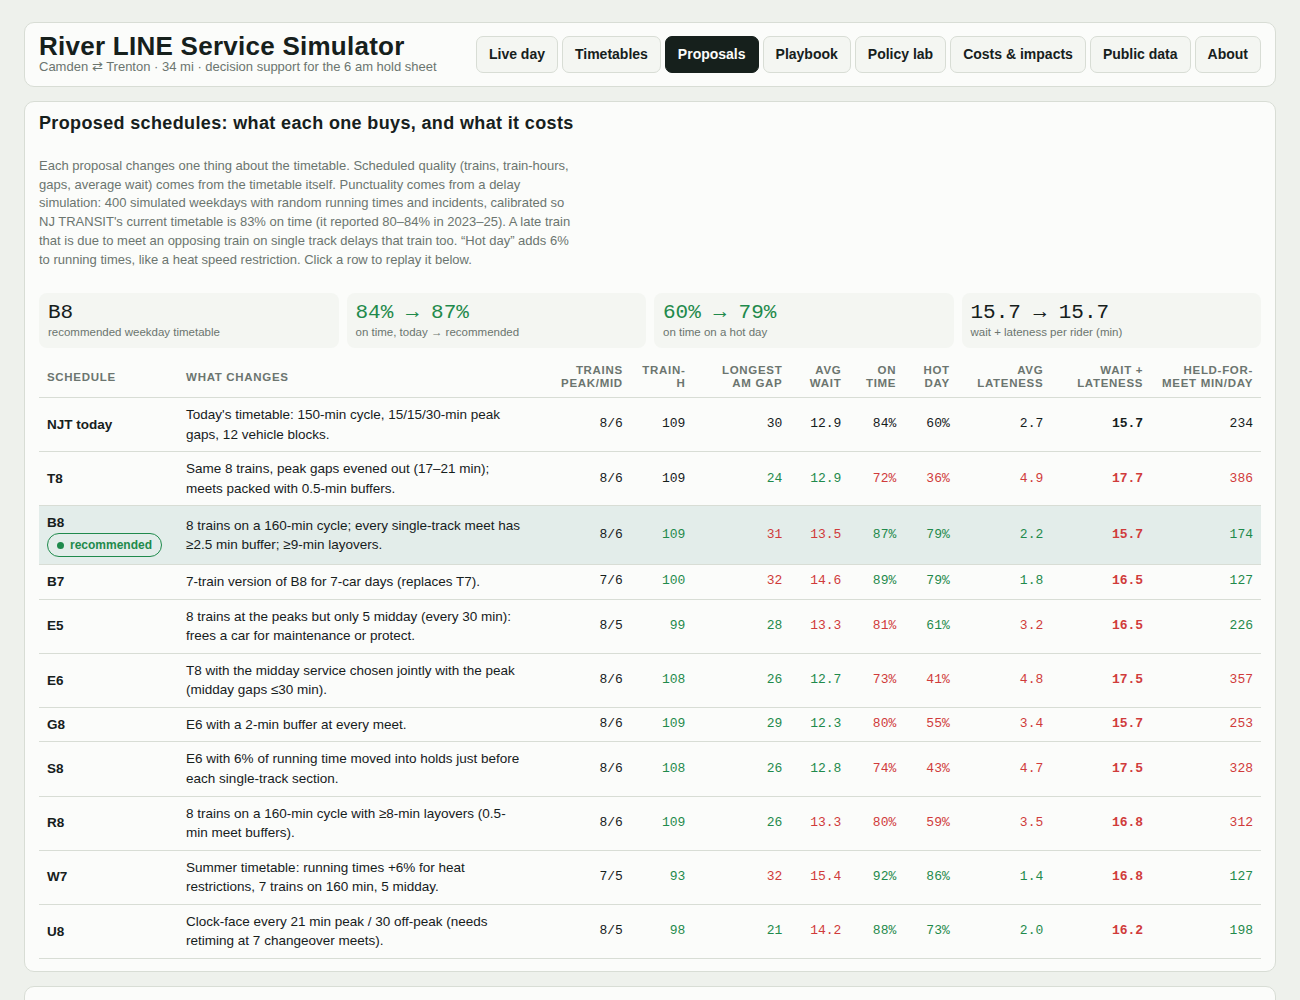
\includegraphics[width=\textwidth]{dash_prop.png}\\[4pt]
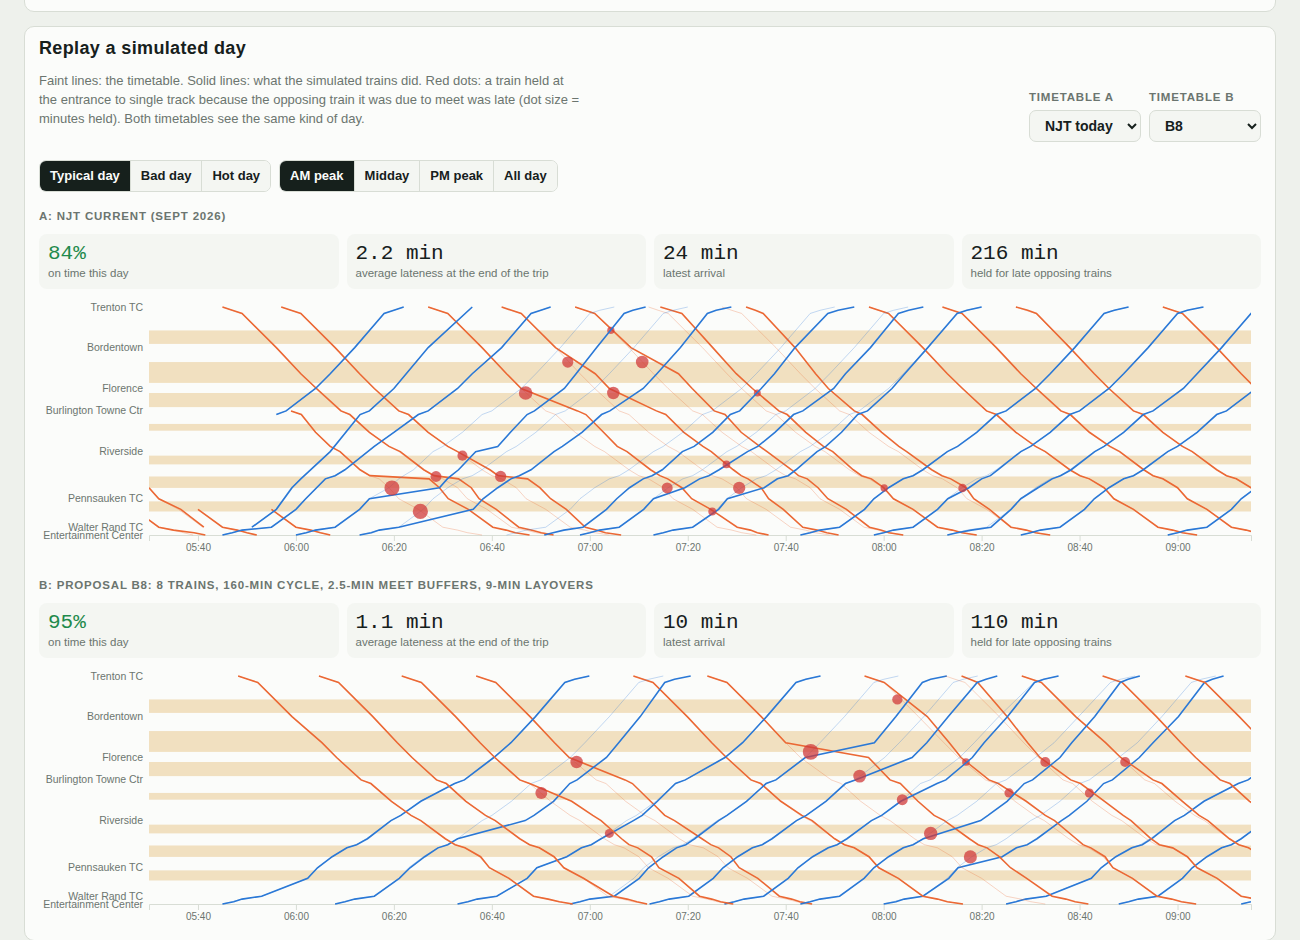
\includegraphics[width=\textwidth]{dash_replay.png}
\caption{Dashboard, Proposals tab: the comparison table (top) and the replay of a simulated morning under today's timetable and B8 (bottom).}\label{fig:dashprop}
\end{figure}

%======================================================================
\section{Costs and effects not yet accounted for}\label{sec:gaps}
\begin{table}[ht]\centering\small
\begin{tabularx}{\textwidth}{@{}p{4.3cm}p{1.5cm}L@{}}
\toprule
Cost or effect & Status & Notes and source for a first estimate \\
\midrule
Train operating cost & Modeled & Assumed \$400/train-hour; NTD 2024 averages \$560--809 \citep{ntd_metrics}. \\
Rider waiting time & Modeled & Equation~\eqref{eq:wait}; USDOT value of time \citep{usdot2016vtts}. \\
Unplanned cancellations; rescues & Modeled & Extra weight on unexpected wait; rescue ties up a second car. \\
Single-track blockages & Partly & Fixed blockage time in the fleet simulation. \\
Knock-on delays at meets; recovery in layovers & Modeled & Delay simulation (Section~\ref{sec:delaymodel}); not yet combined with breakdowns \citep{olsson2004influencing}. \\
Crowding and comfort & Partly & 184 per car (90 seated) \citep{njdot2021riverline}; trip-level counts are needed. \\
Bus bridge & Partly & NTD 2024 NJT bus \$126--214 per hour \citep{ntd_metrics}. \\
Ridership response & Not yet & Frequency elasticities in TCRP Report 95 \citep{evans2004tcrp95ch9}. \\
Repair prioritization; shop capacity & Not yet & Links to maintenance routing \citep{maroti2005maintenance}. \\
Operator availability & Not yet & Crews may bind before cars do. \\
Transfers at the ends & Not yet & 38\% of 2010 riders left the River LINE by transit \citep{dvrpc2013riverline}. \\
Rider communication; events; equity & Not yet & 6\,am publication; waterfront concerts; Camden and Trenton neighborhoods. \\
\bottomrule
\end{tabularx}
\caption{Coverage of costs and effects.}\label{tab:gaps}
\end{table}

%======================================================================
\section{Conclusions}
\begin{enumerate}
\item \textbf{One measure, one ranking.} On reliable trip-miles delivered, the robust timetable B8 (or robust tiers when cars are short) beats today's timetable by 3--5 points in every calibrated scenario, at the same cost (Section~\ref{sec:combined}).
\item \textbf{Fleet reliability is the biggest lever.} The 2026 recovery is worth 13--18 points. No schedule reaches the proposed 90\% target without a more reliable fleet.
\item \textbf{The single track sets the menu, and today's timetable already exploits it.} NJ TRANSIT's 15/15/30 peak runs 8 trains where even spacing would need 9. Calibrating the track model to NJ TRANSIT's own meets was needed to see this.
\item \textbf{With 8 trains, even spacing and punctuality trade off.} T8 narrows the largest morning gap from 30 to 21 minutes with the same trains, but on-time performance falls from 84\% to 72\% because its meets and layovers have no slack. Today's irregular timetable is, in effect, buying recovery time.
\item \textbf{A robust 8-train timetable beats today's on punctuality at no extra cost.} B8 (2.5-minute meet buffers, 9-minute layovers, 160-minute cycle) is on time 87\% (79\% on hot days, against 60\%) with the same trains and train-hours, under every delay assumption we tried.
\item \textbf{Summer timetable: only if heat restrictions are confirmed.} W7 keeps 86\% on time on hot days but runs fewer trips. It loses on the combined measure, and our heat model overstates bad days.
\item \textbf{A ladder of conflict-free timetables for 3--8 trains is ready to review.} It is printed in the Timetable Book.
\item \textbf{On short days, a smaller published timetable beats a large one run with gaps.} With 5--8 cars, the matching tier with protect cars keeps cancellations near 2--4\%, against 7--40\% when today's timetable is run with whatever cars are available. Use B7 in place of T7; T8 is not recommended.
\item \textbf{How much this matters depends on fleet reliability.} If reliability recovers, today's timetable is fine. The hold sheets decide.
\end{enumerate}

%======================================================================
\section{Future work and to-do list}
\paragraph{Validation (first priority).}
\begin{itemize}
\item Get train-level cancellation and arrival records for 2024--26. They settle the one unresolved test (cancellations) and let us refit repair times.
\item Replace the all-day +6\% hot-day assumption with observed heat speed restrictions (hours and segments), and refit so the worst summer days match 45--56\%.
\item Add a ridership response to RTD, using the 2026 recovery (+12--22\%) as a first calibration point.
\item Agree the targets of Section~\ref{sec:glance} with NJ TRANSIT.
\end{itemize}
\paragraph{Data (weeks 1--4).}
\begin{itemize}
\item Obtain the hold sheets, failure logs, and official track chart (Data Request priorities 1--2).
\item Replace the calibrated siding positions with the official ones.
\item Fit failure rates against temperature.
\end{itemize}
\paragraph{Models (weeks 4--10).}
\begin{itemize}
\item \textbf{Validate the delay model.} Fit running-time variation, incidents and dwell times to train-level arrival records, and check the calibration of 83\% on time against NJ TRANSIT's own figures by month.
\item \textbf{Optimize robustness directly.} Instead of sweeping buffer and layover sizes, maximize the minimum (or expected) slack at meets subject to a bound on waiting, in the spirit of light robustness \citep{fischetti2009light}, or optimize the supplements with the simulation in the loop \citep{kroon2008stochastic}. There may be 8-train timetables that are both more even and more punctual than B8.
\item \textbf{Combine the two simulations.} Breakdowns, rescues and knock-on delays in one engine, so cancellations and lateness are counted together.
\item \textbf{Whole-day timetable model.} Retime the changeovers of the uniform tiers so that they are conflict-free all day.
\item \textbf{Two-stage stochastic tier selection.} Choose which tiers to publish before the day, then pick one at 6\,am, evaluated with recoverable robustness \citep{liebchen2009concept}; add the 6\,pm hold sheet as a second decision point.
\item \textbf{Richer objective.} Add crowding, transfers, and ridership response \citep{evans2004tcrp95ch9}.
\end{itemize}
\paragraph{Deliverables (weeks 8--14).}
\begin{itemize}
\item Export each tier as GTFS for NJ TRANSIT's scheduling system.
\item Build a one-page hold-sheet form that feeds the playbook.
\item Hand over the dashboard with calibrated parameters. Use open-source tools (HiGHS) throughout, so NJ TRANSIT can run the model without academic-only licenses.
\end{itemize}

\bibliographystyle{plainnat}
\bibliography{refs}

\appendix
\section{Model parameters}
\begin{table}[ht]\centering\small
\begin{tabularx}{\textwidth}{@{}p{4.6cm}p{3.2cm}L@{}}
\toprule
Parameter & Value & Basis \\
\midrule
Fleet; cars in long-term overhaul & 20; 3 & \citet{wiki_riverline}; assumption \\
Miles between breakdowns & 4{,}192 & \citet{roinj2025riverline} \\
Seasonal multipliers (breakdown miles) & W 0.85, Sp 1.25, Su 0.65, F 1.0 & Placeholder; client notes; \citet{ferranti2016heat} \\
Mean repair time & 12 days & Placeholder \\
Rescue: dispatch, speed, couple, tow & 10 min, 25 mph, 10 min, 15 mph & Placeholders \\
Single-track blockage & 35 min & Placeholder \\
Minimum turnback; meet buffer & 5 min; 0.5 min & GTFS blocks; calibration \\
Track calibration & +1.5 mi north of MP 12 & Fit to 213 scheduled meets (Section~\ref{sec:calib}) \\
Running times & 67 min each way & GTFS Sept.~2026 medians \citep{njt2026gtfs} \\
Weekday boardings & 5{,}600 & \citet{wiki_riverline} \\
Train-hour cost; value of time & \$400 (rev.~2); \$547 (rev.~4); \$13.60/h ($\times 2$) & \$547 = NTD FY2024 vehicle operations + maintenance per revenue hour \citep{ntd_ts21}; \citet{usdot2016vtts} \\
Calibrated scenarios (rev.~4) & S1: MDBF 3{,}661, repairs 10 d; S2: 3{,}568, 5 d; S3: 10{,}000, 5 d & \citet{njt_mdbf}; Section~\ref{sec:combined} \\
Delay model: supplement; noise (trip, segment) & 10\%; lognormal s.d.\ 0.035, 0.12 & Assumption; sensitivity in Figure~\ref{fig:propsens} \\
Delay model: incidents & 0.21 per trip, mean 6 min & Fitted to 83\% on time \citep{roinj2025riverline} \\
Hot day; turnaround; on-time limit & +6\% running time; 3 min; $<$6 min late & Assumption; \citet{njt2019otp} \\
\bottomrule
\end{tabularx}
\end{table}


\section{Sweep of robust 8-train patterns}\label{app:sweep}
\begin{table}[ht]\centering\small
\begin{tabular}{@{}rrrrrrrrr@{}}
\toprule
Cycle & Meet buffer & Min.\ layover & Train- & Longest & Avg & On time & Hot day & Wait + \\
(min) & (min) & (min) & hours & AM gap & wait & (\%) & (\%) & lateness \\
\midrule
150 & 1.5 & 7 & 109 & 30 & 12.5 & 80 & 55 & 16.0 \\
150 & 2 & 6.5 & 109 & 30 & 12.5 & 80 & 55 & 15.9 \\
155 & 1.5 & 8 & 106 & 30 & 13.6 & 84 & 69 & 16.5 \\
155 & 2 & 8 & 107 & 30 & 13.4 & 85 & 66 & 16.0 \\
160 & 2 & 8 & 108 & 27 & 13.5 & 85 & 69 & 16.3 \\
160 & 1.5 & 10 & 107 & 25 & 13.7 & 78 & 56 & 17.8 \\
165 & 2 & 10 & 108 & 32 & 13.3 & 86 & 75 & 15.6 \\
160 & 2.5 & 9 & 109 & 31 & 13.5 & 87 & 79 & 15.7 \\
\bottomrule
\end{tabular}
\caption{8-train patterns with 6 midday trains, 300 simulated days each. B8 is the 160 / 2.5 / 9 row. For reference, today's timetable: 84\% and 60\% on time, wait + lateness 15.7 minutes.}\label{tab:sweep}
\end{table}

\section{Reproducing the results}
\begin{itemize}
\item \texttt{python analysis/calibrate\_track.py} --- track calibration.
\item \texttt{python analysis/run\_patterns.py} --- pattern timetables, about 15 minutes.
\item \texttt{python analysis/proposals\_solve.py}, \texttt{robust\_sweep.py}, \texttt{robust\_b7.py} --- pattern MIPs for the proposals (about 30 minutes on 2 cores).
\item \texttt{python analysis/timetable\_build.py} --- full-day timetables, metrics, CSVs, and the timetable book.
\item \texttt{python analysis/delay\_eval.py} --- delay simulation of every timetable, sensitivity runs, and dashboard replays.
\item \texttt{python analysis/proposal\_figs.py} --- figures and tables of Section~\ref{sec:prop}.
\item \texttt{python analysis/delay\_regimes.py}, \texttt{combined\_eval.py}, \texttt{combined\_figs.py} --- Section~\ref{sec:combined} (the combined runs use the dashboard engine through \texttt{rl\_map/jsrun.py}).
\item \texttt{python src/run\_all.py} --- uniform ladder.
\item \texttt{python analysis/public\_analysis.py} --- public-data figures.
\item \texttt{python analysis/report\_figs.py} --- report figures from the dashboard engine's results (\texttt{results/js\_eval.json}).
\end{itemize}
The timetables are also in \texttt{timetables/*.csv}.
\end{document}
